\section*{\textbf{Appendix}}

\section{Additional results on noisy small scale models} \label{app:noisy}

Refer to Fig. \ref{fig:motivation_app}.

\begin{figure}[htb]
    \centering

    \begin{subfigure}[b]{0.497\textwidth}
        \centering
        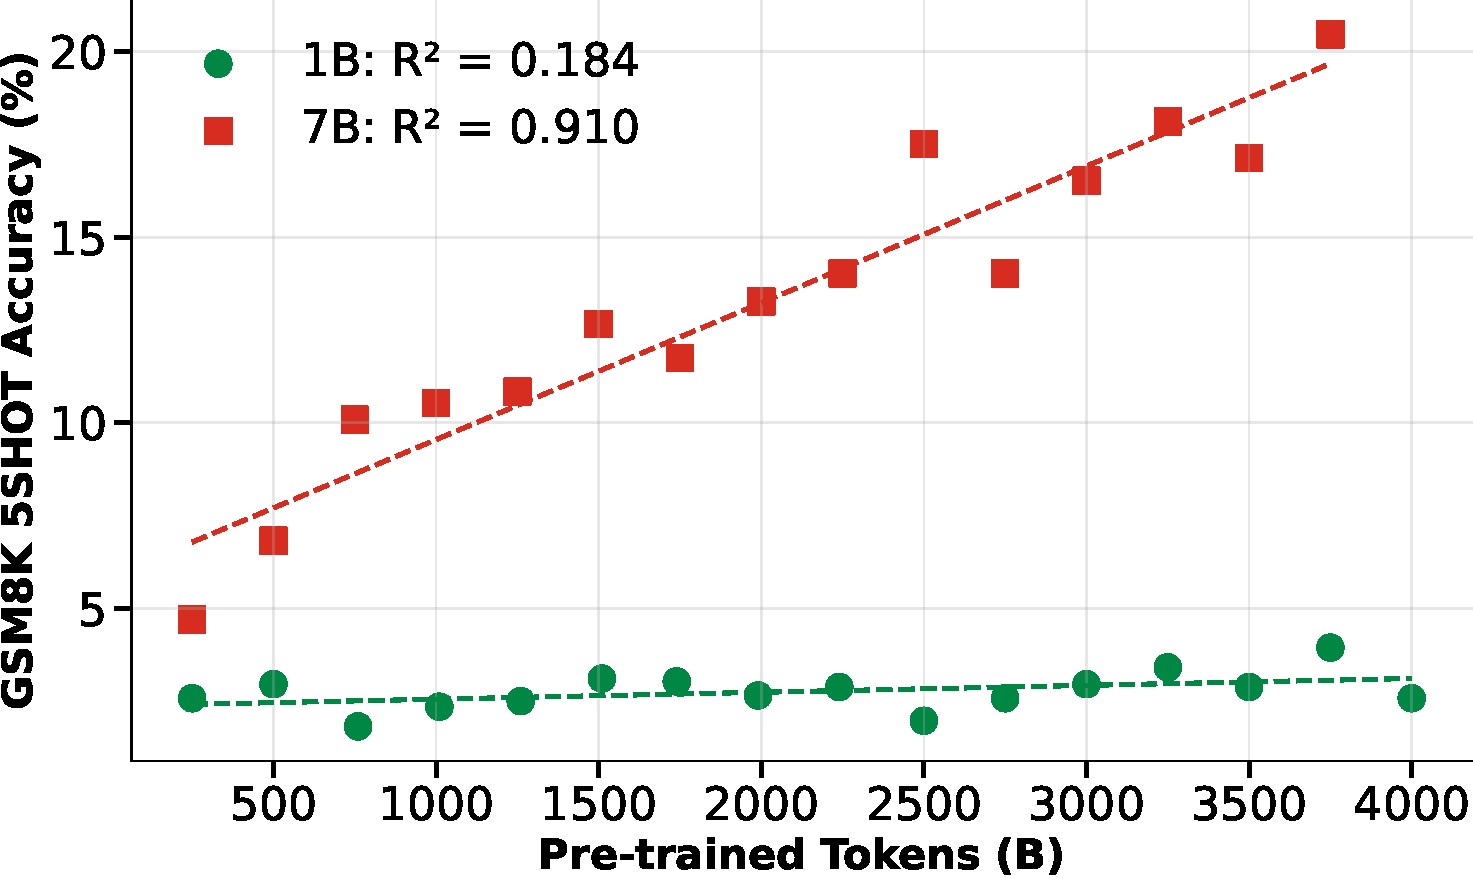
\includegraphics[width=\textwidth]{figs/gsm8k_5shot_1b_7b_performance.pdf}
    \end{subfigure}
    \hfill
    \begin{subfigure}[b]{0.497\textwidth}
        \centering
        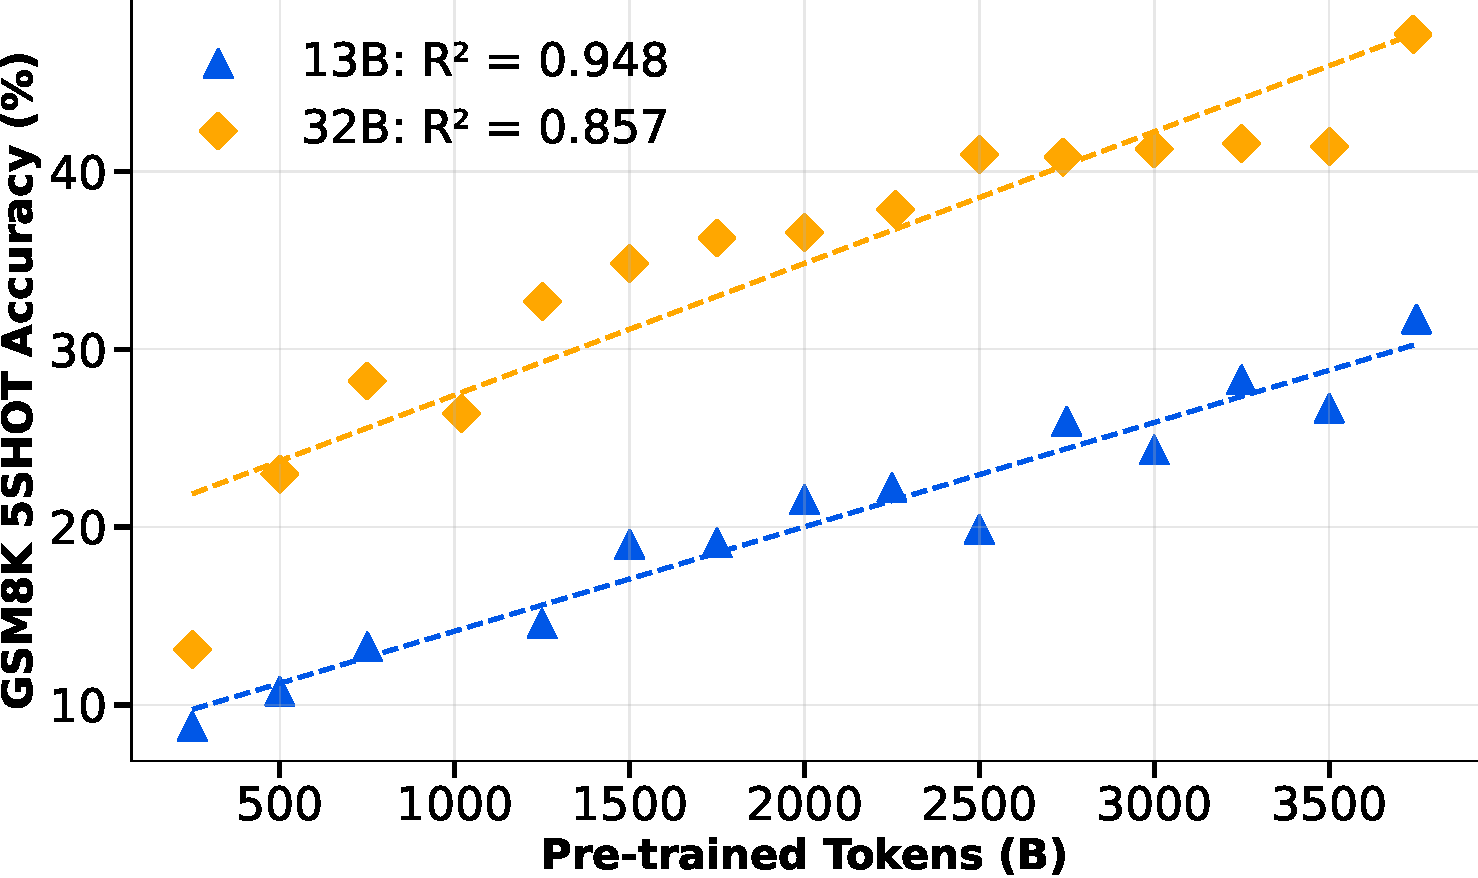
\includegraphics[width=\textwidth]{figs/gsm8k_5shot_13b_32b_performance.pdf}
    \end{subfigure}

    \begin{subfigure}[b]{0.497\textwidth}
        \centering
        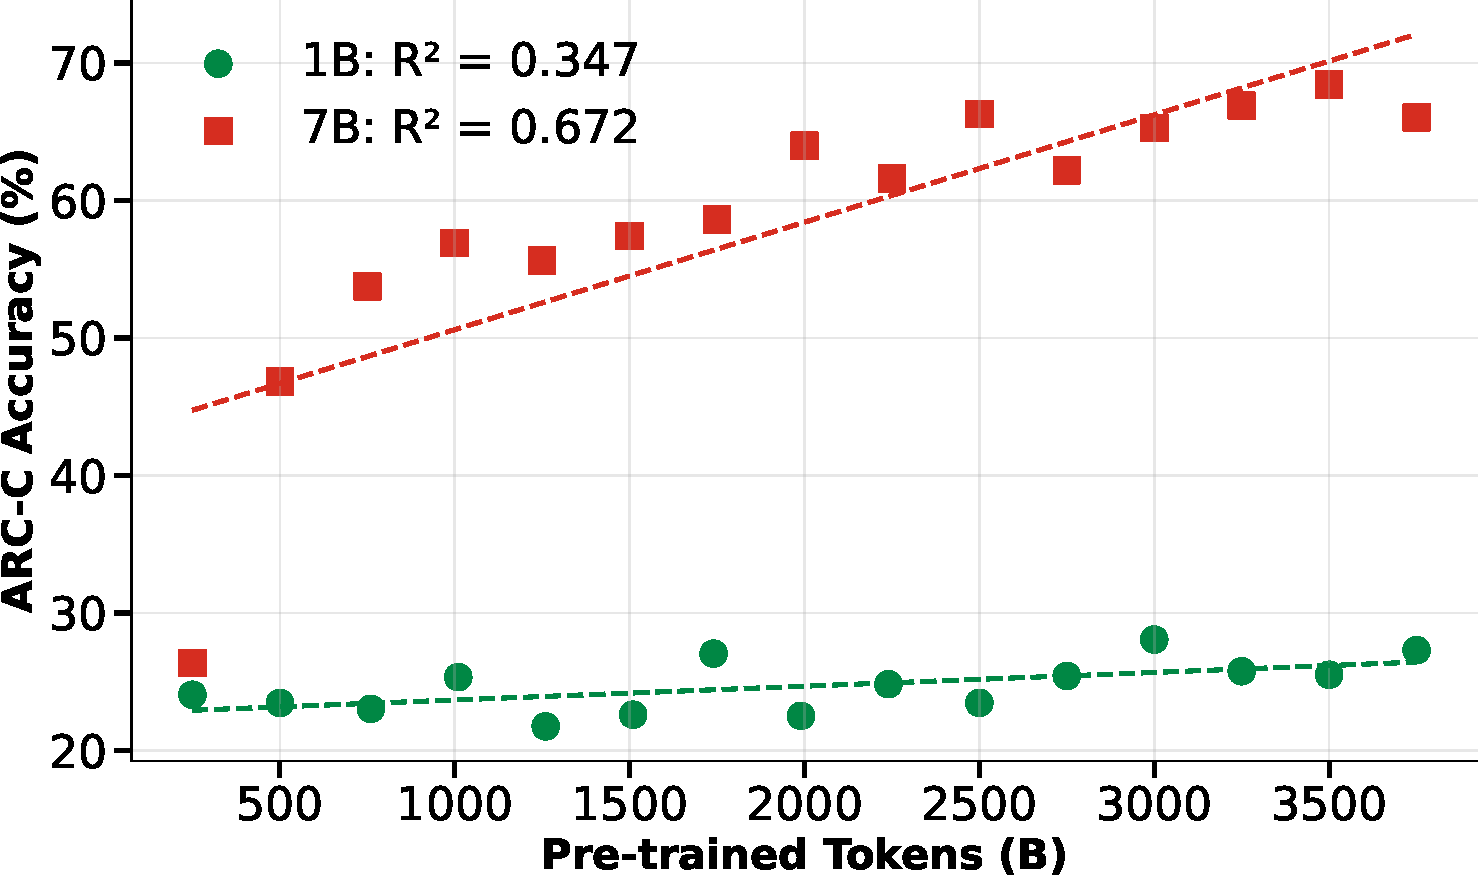
\includegraphics[width=\textwidth]{figs/arc-c_1b_7b_performance.pdf}
    \end{subfigure}
    \hfill
    \begin{subfigure}[b]{0.497\textwidth}
        \centering
        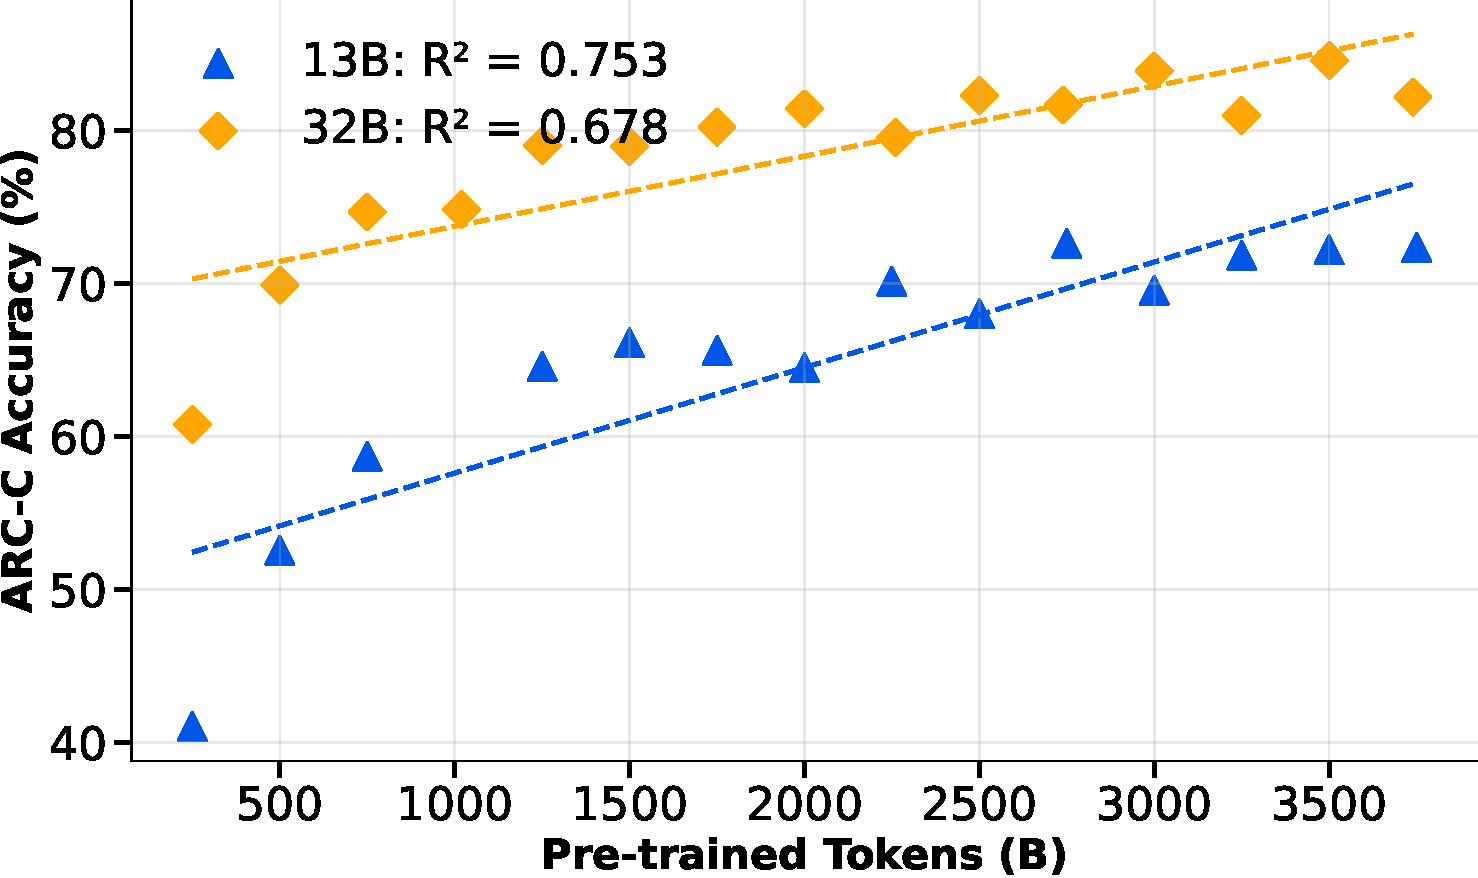
\includegraphics[width=\textwidth]{figs/arc-c_13b_32b_performance.pdf}
    \end{subfigure}

    \begin{subfigure}[b]{0.497\textwidth}
        \centering
        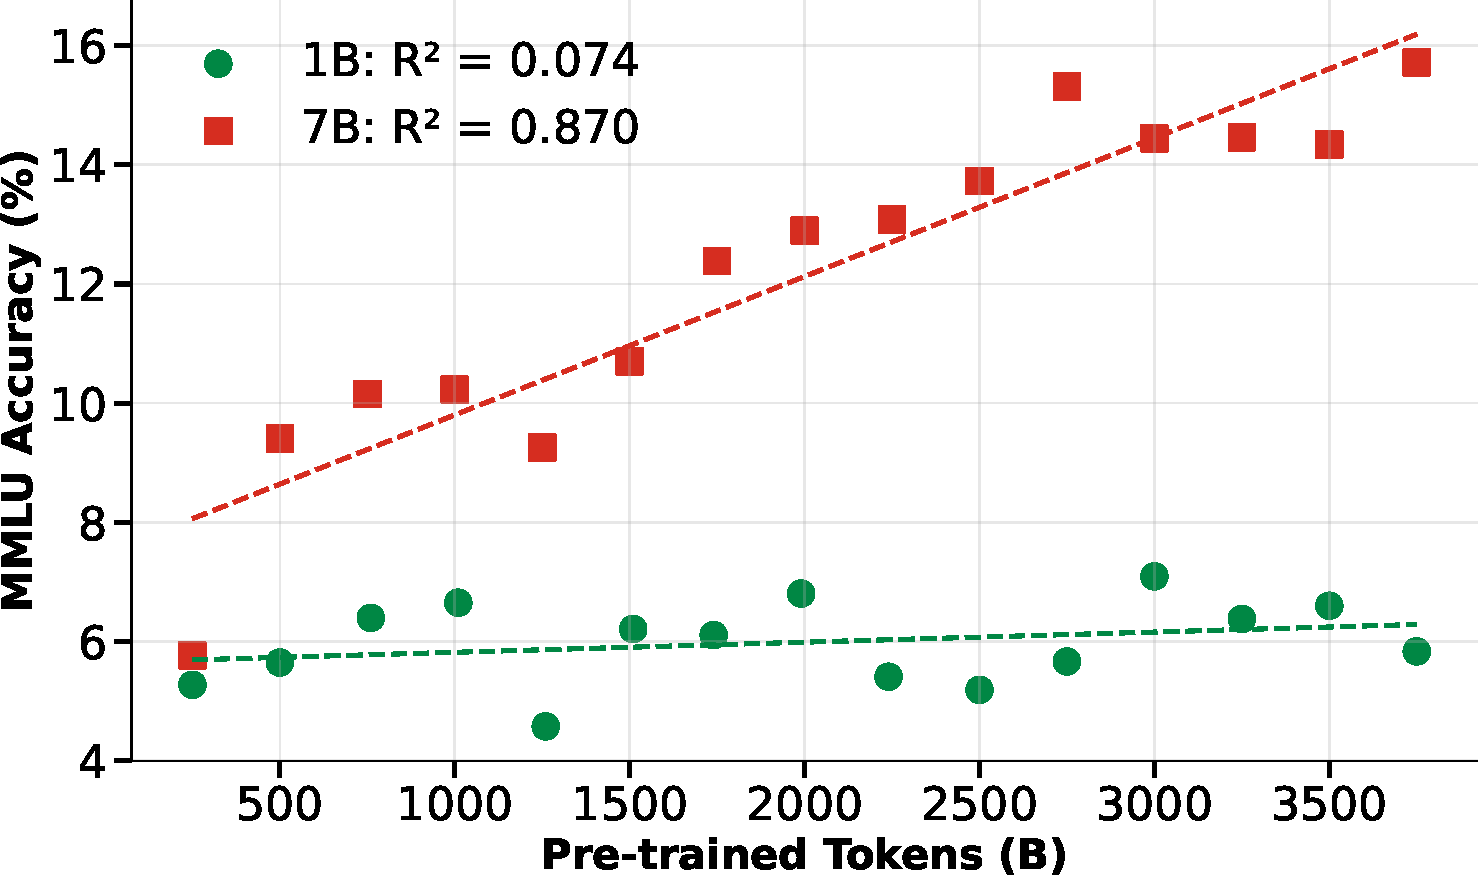
\includegraphics[width=\textwidth]{figs/mmlu_1b_7b_performance.pdf}
    \end{subfigure}
    \hfill
    \begin{subfigure}[b]{0.497\textwidth}
        \centering
        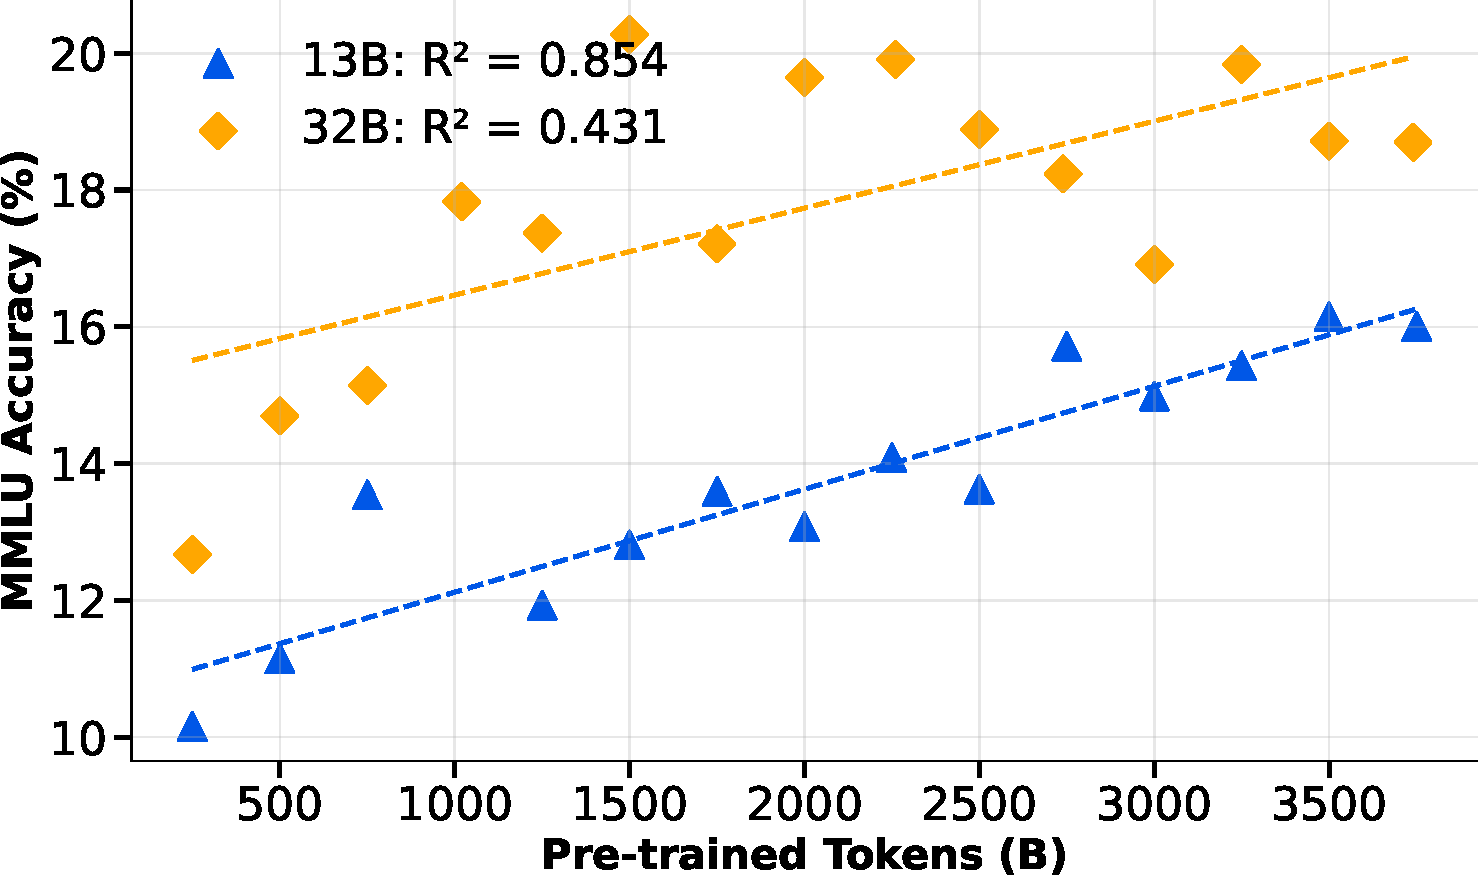
\includegraphics[width=\textwidth]{figs/mmlu_13b_32b_performance.pdf}
    \end{subfigure}
    
    \begin{subfigure}[b]{0.497\textwidth}
        \centering
        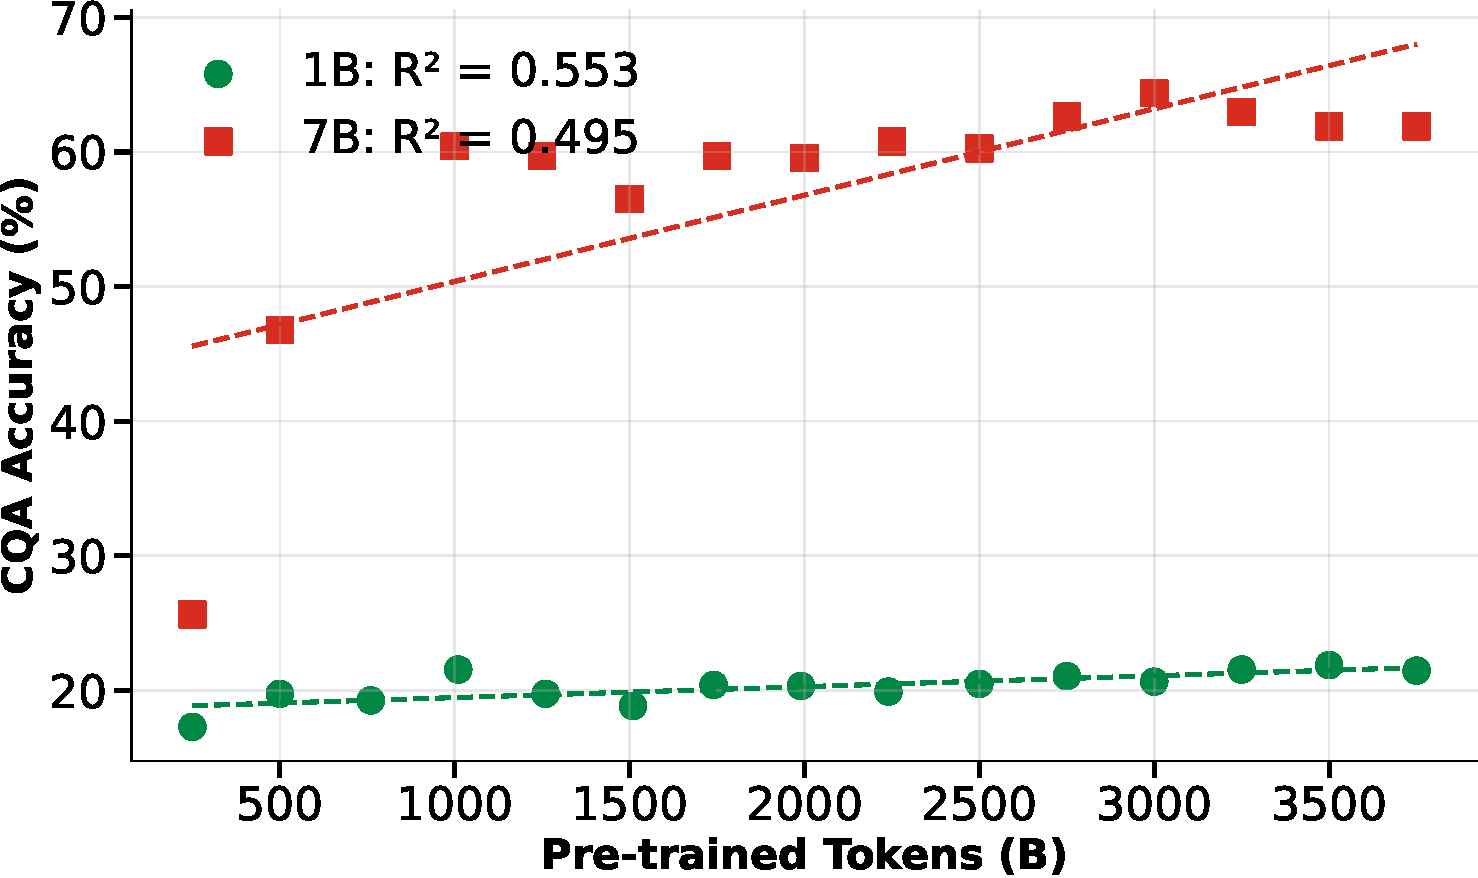
\includegraphics[width=\textwidth]{figs/cqa_1b_7b_performance.pdf}
    \end{subfigure}
    \hfill
    \begin{subfigure}[b]{0.497\textwidth}
        \centering
        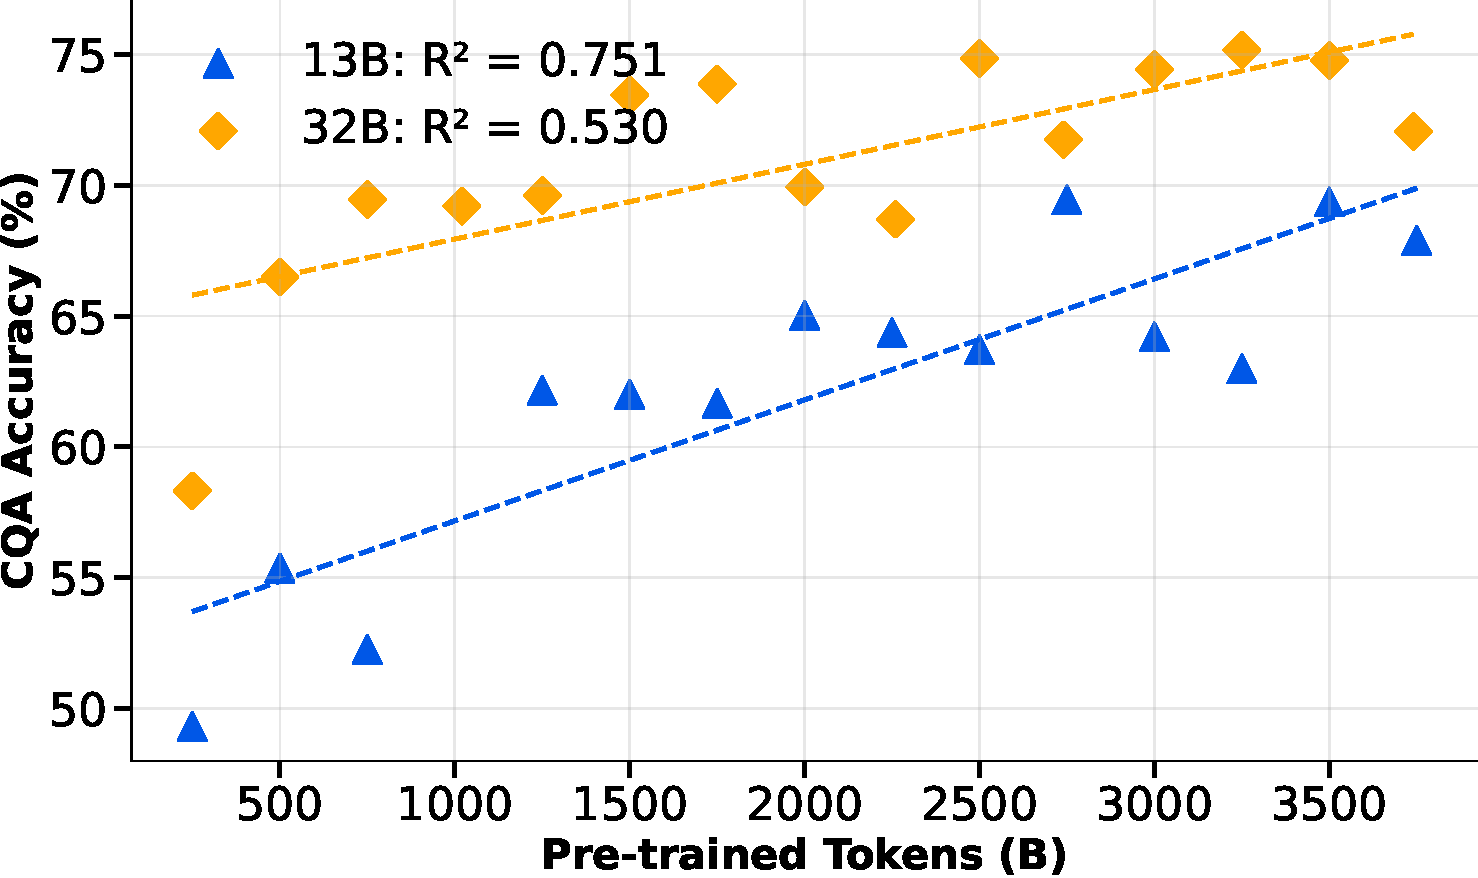
\includegraphics[width=\textwidth]{figs/cqa_13b_32b_performance.pdf}
    \end{subfigure}

\begin{subfigure}[b]{0.497\textwidth}
        \centering
        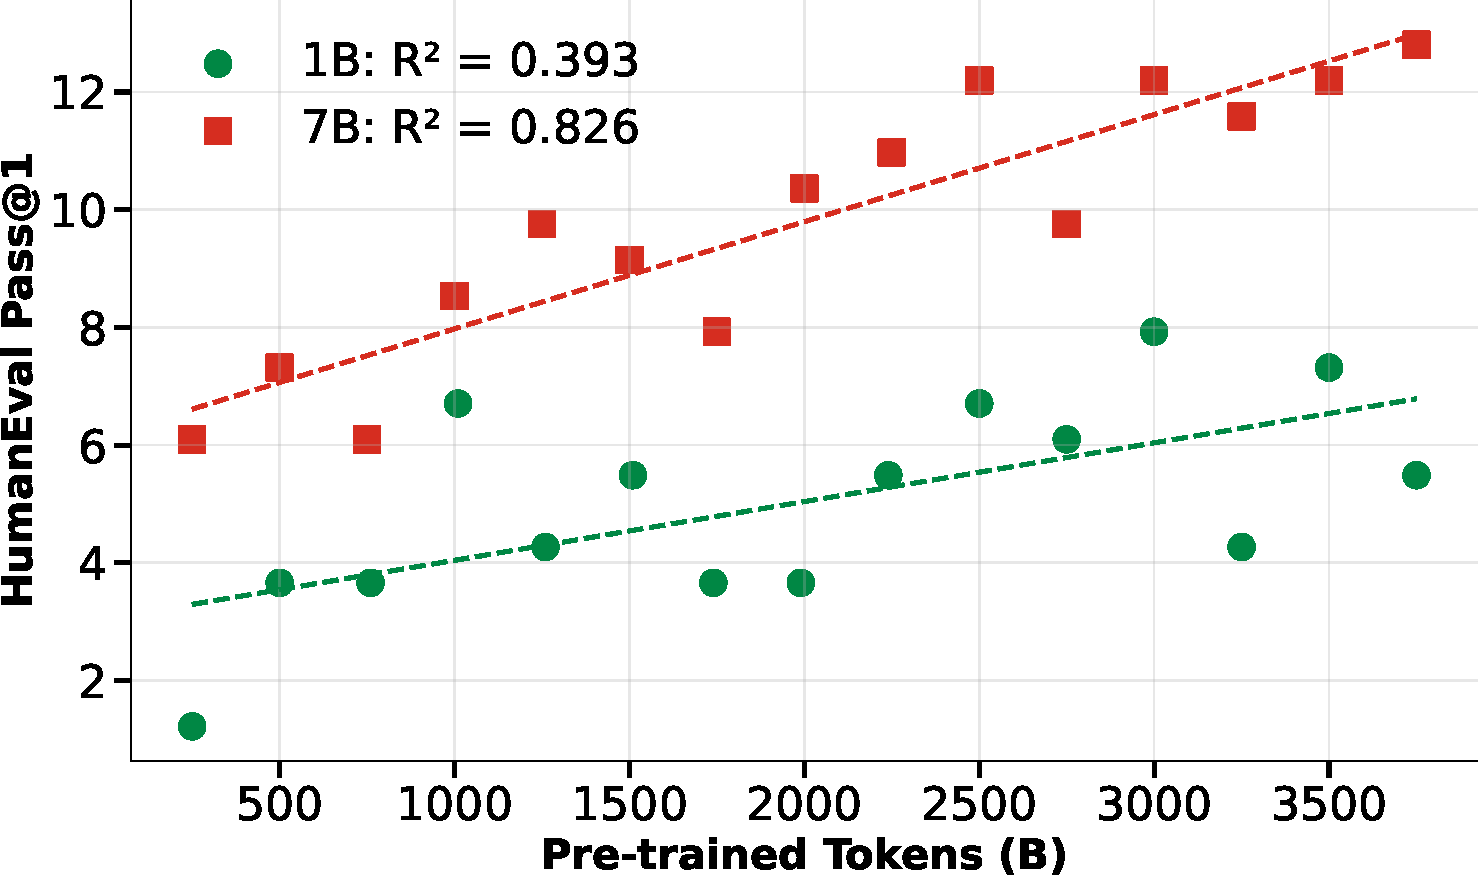
\includegraphics[width=\textwidth]{figs/humaneval_1b_7b_performance.pdf}
        \caption{Pre-training progress on 1B and 7B model}
    \end{subfigure}
    \hfill
    \begin{subfigure}[b]{0.497\textwidth}
        \centering
        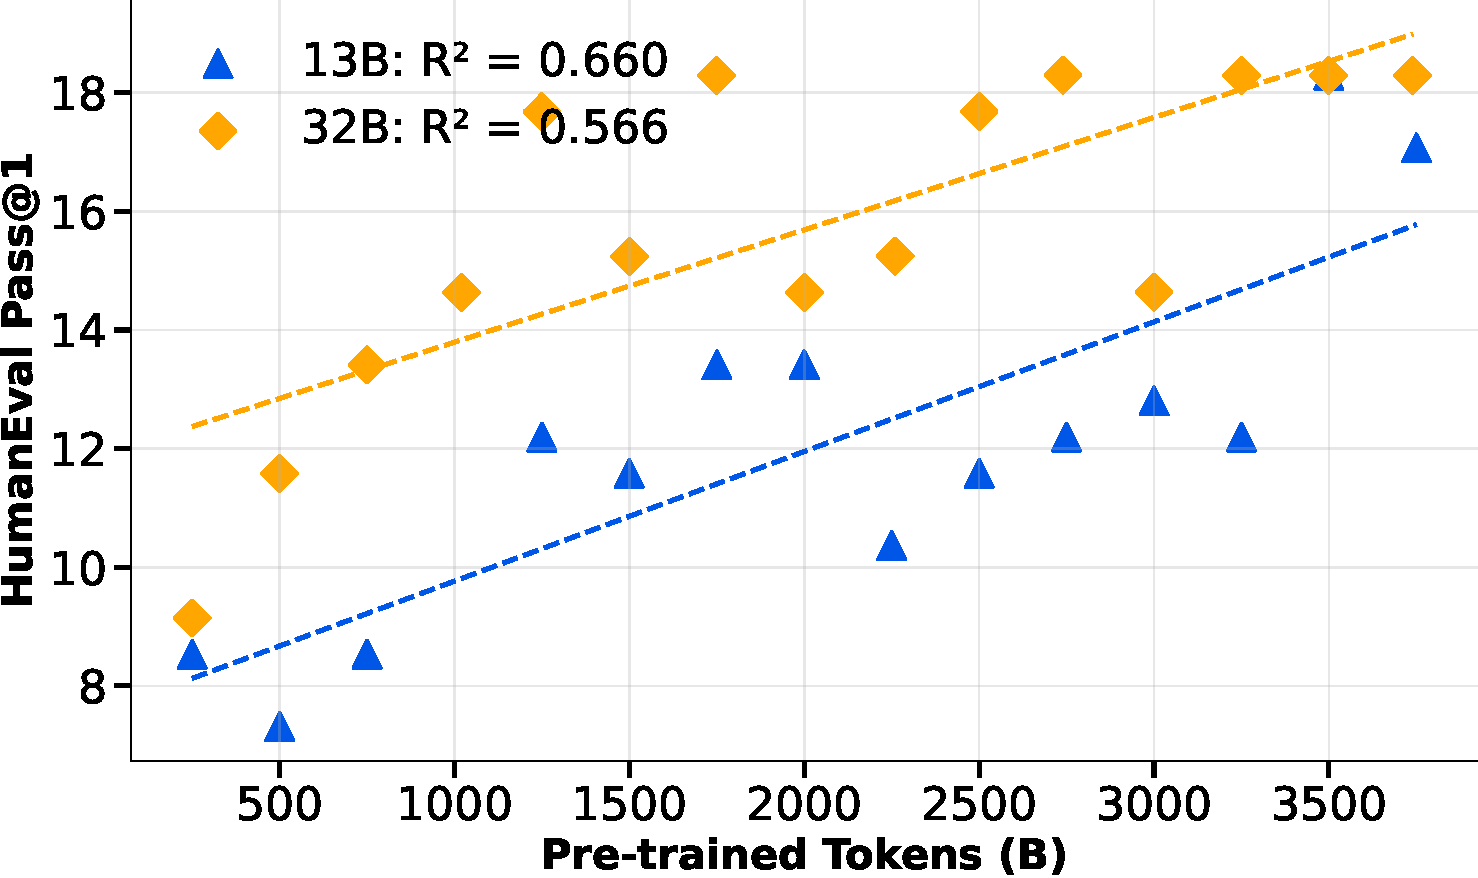
\includegraphics[width=\textwidth]{figs/humaneval_13b_32b_performance.pdf}
        \caption{Pre-training progress on 13B and 32B model}
    \end{subfigure}
    
    \caption{Given the same data source, smaller models exhibit significantly more noise and occasionally provide the wrong direction, making it challenging to use smaller models to proxy larger model performance. R$^2$ values are derived from linear curve fitting. MMLU corresponds to MMLU Pro (STEM).}
    \label{fig:motivation_app}
\end{figure}

\section{rBridge Pseudocode} \label{app:pseudocode}

\paragraph{Pseudocode.} The pseudocode is available in Alg. \ref{alg:rbridge}. We recommend viewing with Fig. \ref{fig:rbridge} to build intuition. Recall that $x$ is an input from the benchmark dataset's validation or test we want to evaluate. Recall that $\pi^\text{p}, \pi^\phi$ are the proxy, and frontier LMs, respectively. $i$ denotes index of token $\tau$. $\tau^\text{p}$ denotes the token tokenized using $\pi^\text{p}$'s tokenizer. Exact prompt and extraction used in Line 1 is available in \hyperlink{prompt}{prompt}.

\SetKwInput{Input}{Input}
\SetKwInput{Return}{Return}

\begin{algorithm2e}[H]
    \caption{\tsc{rBridge}}
    \label{alg:rbridge}
    \Input{$x, \pi^\text{p}, \pi^\phi$}
        \tcc{Step 1: Extract reasoning trace and token-level confidence from frontier model}
     $R^\phi, p(R^\phi) ,A^\phi \leftarrow \pi^\phi(x)$ \;

    \tcc{Step 2: Discard answer label, and compute normalized \tsc{rBridge} NLL}
    $w \leftarrow []$\;
    \For{\textnormal{\textbf{each} \textnormal{token} $\tau_i^\text{p}$ \textnormal{\textbf{tokenizing}} $R^\phi$}}{
       $w_i \leftarrow $\textnormal{Mean} $_{\text{letter} \in \tau_i^\text{p}}(p^\phi($\textnormal{letter}$)$ \textnormal{from} $p(R^\phi))$ \;
        $w.\text{append}(w_i)$
    }
    \tsc{rBridge} $\leftarrow []$\;
    \For{\textnormal{\textbf{each} \textnormal{token} $\tau_i^\text{p}$ \textnormal{\textbf{tokenizing}} $R^\phi$}}{
       $\textnormal{NLL} \leftarrow-\textnormal{log }p^\text{p}(\tau_i^\text{p}) \sim \pi^\text{p}$ \;
        \tsc{rBridge}.append$(\text{NLL}\cdot\frac{w[i]-\text{min}(w)}{\text{max}(w)-\text{min}(w)})$\;
    }
    \tsc{rBridge} $\leftarrow \text{Mean}(\tsc{rBridge})$\;
    \Return{\tsc{rBridge}}
\end{algorithm2e}


\paragraph{Prompt.} Here is the \hyperlink{prompt}{prompt} we use to generate $R^\phi$. We use greedy decoding. Brackets [] indicate dynamic insertions depending on the benchmark and question. We extract the value for key ``reasoning" to attain $R^\phi$.

\hypertarget{prompt}{}
\begin{tcolorbox}[colback=gray!5!white, colframe=gray!75!black, title=Prompt to Frontier Model, label={box:mailman_question}]

System: You are a helpful assistant that solves [task] problems.

\vspace{1em}

User: [question]

Respond ONLY with a JSON object in this exact format:
\{ ``reasoning": ``your step by step reasoning", ``final\_answer": ``your final answer" \}

\end{tcolorbox}

\section{Further Experimental Details} \label{app:setting}

\paragraph{Common Evaluation Setting.} All evaluations are done using 5-shot CoT \citep{NEURIPS2022_9d560961}.

\subsection{Hardware} We use A100 80G, H100 and H200 nodes and numerous terabytes of disk storage for experiments. For pre-training, we use 256 H100 GPUs with HBM3. For other hardware like CPU and RAM we use commonly available ones, as these hardware did not induce any bottlenecks. 


\subsection{Experiment (i) Additional Details} All proxy models used is the default seed as provided in \cite{magnusson2025datadecide}. We do not use multi-seed averaging for the proxy as this significantly increases compute cost. We exactly follow  \cite{magnusson2025datadecide} on every other aspect of experiments, using their open-source assets where available. All intermediary checkpoints are as available from \cite{magnusson2025datadecide}.

\subsection{Experiment (ii) Additional Details} 

\paragraph{Additional Baseline Details.} iSFT results are unavailable for MMLU Pro (STEM) and HumanEval as these benchmarks do not provide an SFT set.

\paragraph{Frontier Model's $R^\phi$.} Following \cite{team2025minicpm4}, we use \ttt{GPT 4o} to generate $R^\phi$. We tested \ttt{Claude 3.5 Sonnet} and \ttt{Gemini 2.5 Pro} and found no meaningful performance difference. We have not tested this method on long CoT models.

\paragraph{Pre-training and Post-training Details.} Unless stated otherwise, for pre-training, we fully follow OLMo 2 \citep{olmo20242}, and use their checkpoints where available. For SFT post-training we use the settings in Tab. \ref{tab:hyperparams}.

\begin{table}[ht]
    \centering
    \caption{Hyperparameters for SFT}
    \label{tab:hyperparams}
    \resizebox{0.4\columnwidth}{!}{
        \begin{tabular}{lc}
        \toprule
        \textbf{Hyperparameter} & \textbf{Value} \\
        \midrule
        Epoch & 1 \\
        Learning Rate & $1 \times 10^{-5}$ \\
        Warmup Ratio & 0.1 \\
        Batch Size & 64 \\
        \bottomrule
        \end{tabular}
    }
\end{table}

\subsection{Experiment (iii) Additional Details} 

\paragraph{Alternative Pre-training Dataset $\mc{D}'$.} For the alternative pre-training dataset $\mc{D}'$  described in experiment \textbf{(iii)}, we closely follow the setup described in \cite{han2025trillion}, but exclusively use publicly-available datasets. The training data follows an 8.5:1:0.5 ratio of English:multilingual:math/code, where the English portion consists of DCLM and FineWeb-Edu in equal proportions, and the multilingual portion comprises Korean, Chinese, and Japanese dumps of FineWeb and DCLM pipeline-processed Common Crawl filtered for Korean. 

\paragraph{Benchmark Choice.} We use the same benchmarks presented in \textbf{(ii)}, excluding HumanEval, as our extraction method on the alternative dataset $\mc{D}'$ achieved 0\% p@1.

\section{Additional Experimental Results} \label{app:more_exp}

Refer to Fig. \ref{fig:curve_fit} and \ref{fig:curve_fit_1} for extended curve fitting visualization examples. Refer to Tab. \ref{tab:olmo_1b_13b_pre_to_post} for all 1B $\rightarrow$ 13B (Pre-to-Post) benchmark results. MMLU Pro (STEM) and HumanEval are not included as they do not have a designated SFT set. Refer to Tab. \ref{tab:olmo_1b_32b_pre_to_pre} for all 1B $\rightarrow$ 32B (Pre-to-Pre) benchmark results. Refer to Fig. \ref{fig:kendall} for Kendall Tau results.

\begin{figure}[tb!]
    \centering
    \begin{subfigure}[b]{0.497\textwidth}
        \centering
        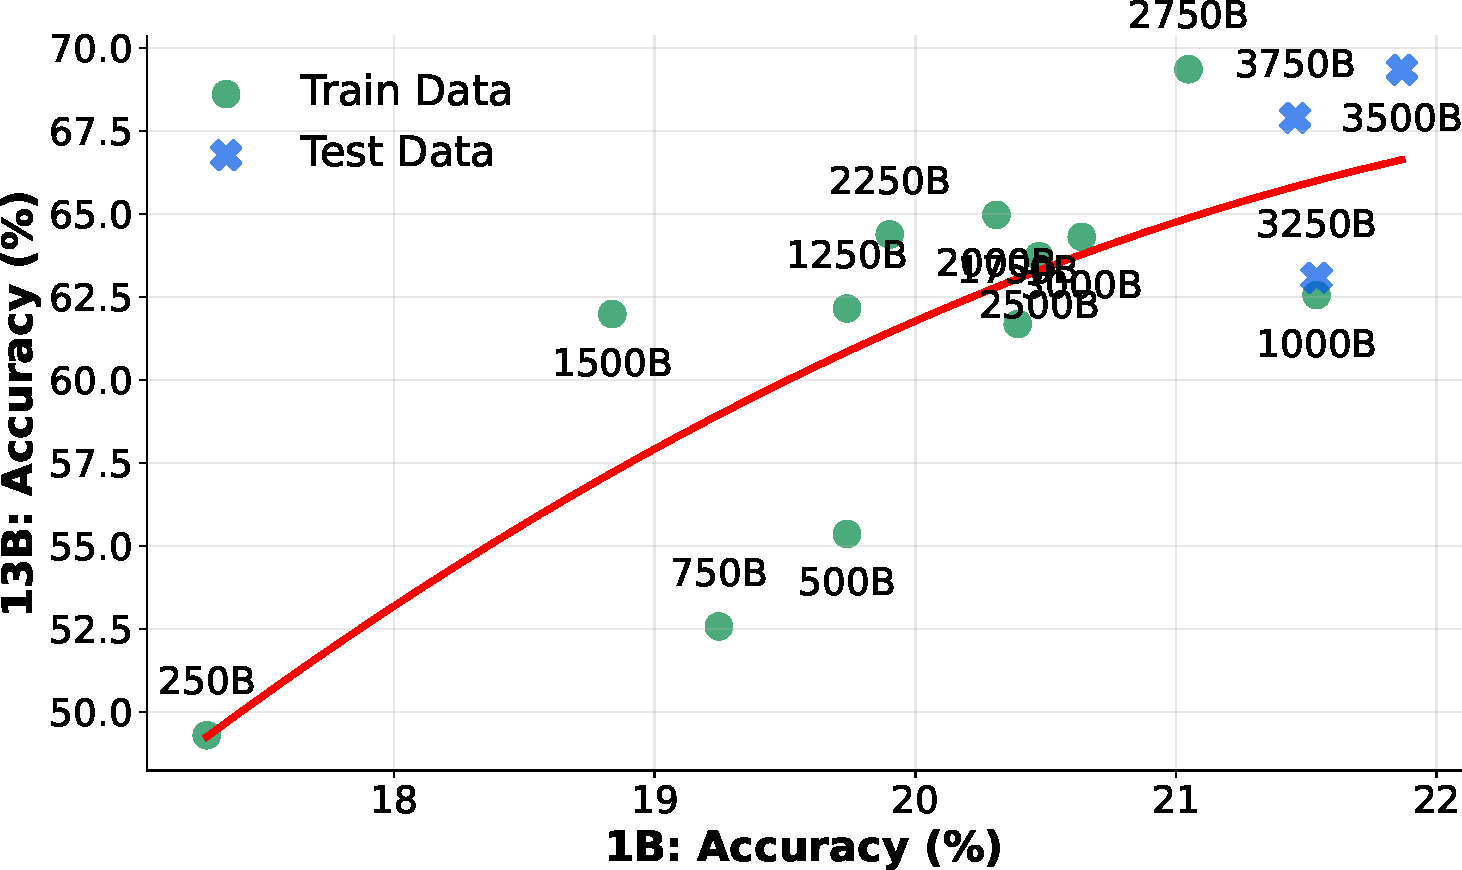
\includegraphics[width=\textwidth]{figs/cqa_acc.pdf}
        \caption{Target metric Acc. as the proxy metric at 1B on CQA.}
    \end{subfigure}
    \hfill
    \begin{subfigure}[b]{0.497\textwidth}
        \centering
        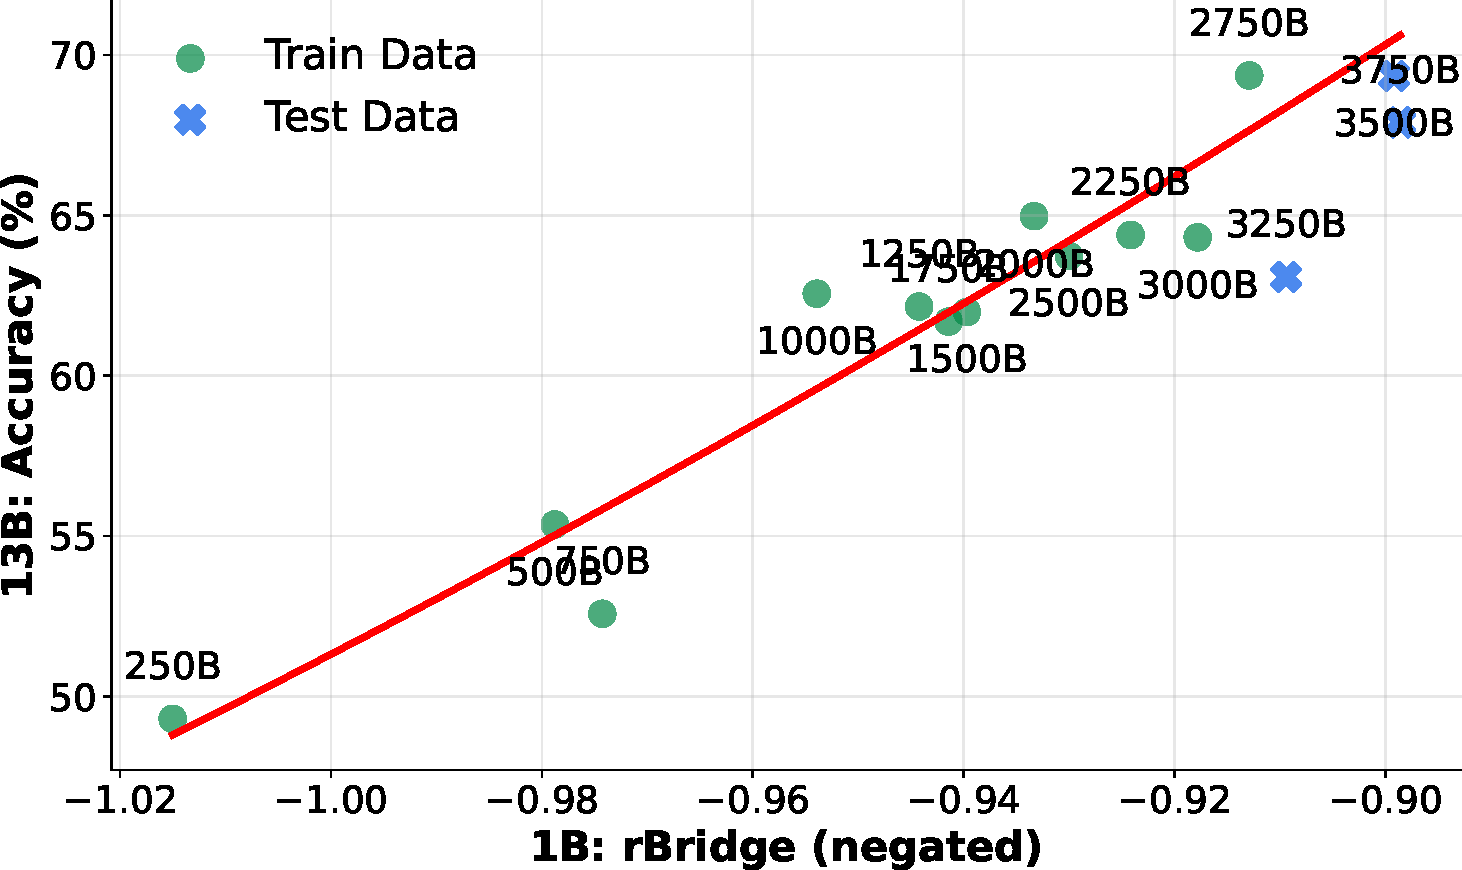
\includegraphics[width=\textwidth]{figs/cqa_rbridge.pdf}
        \caption{\tsc{rBridge} as the proxy metric at 1B on CQA.\\~\\}
    \end{subfigure}

    \begin{subfigure}[b]{0.497\textwidth}
        \centering
        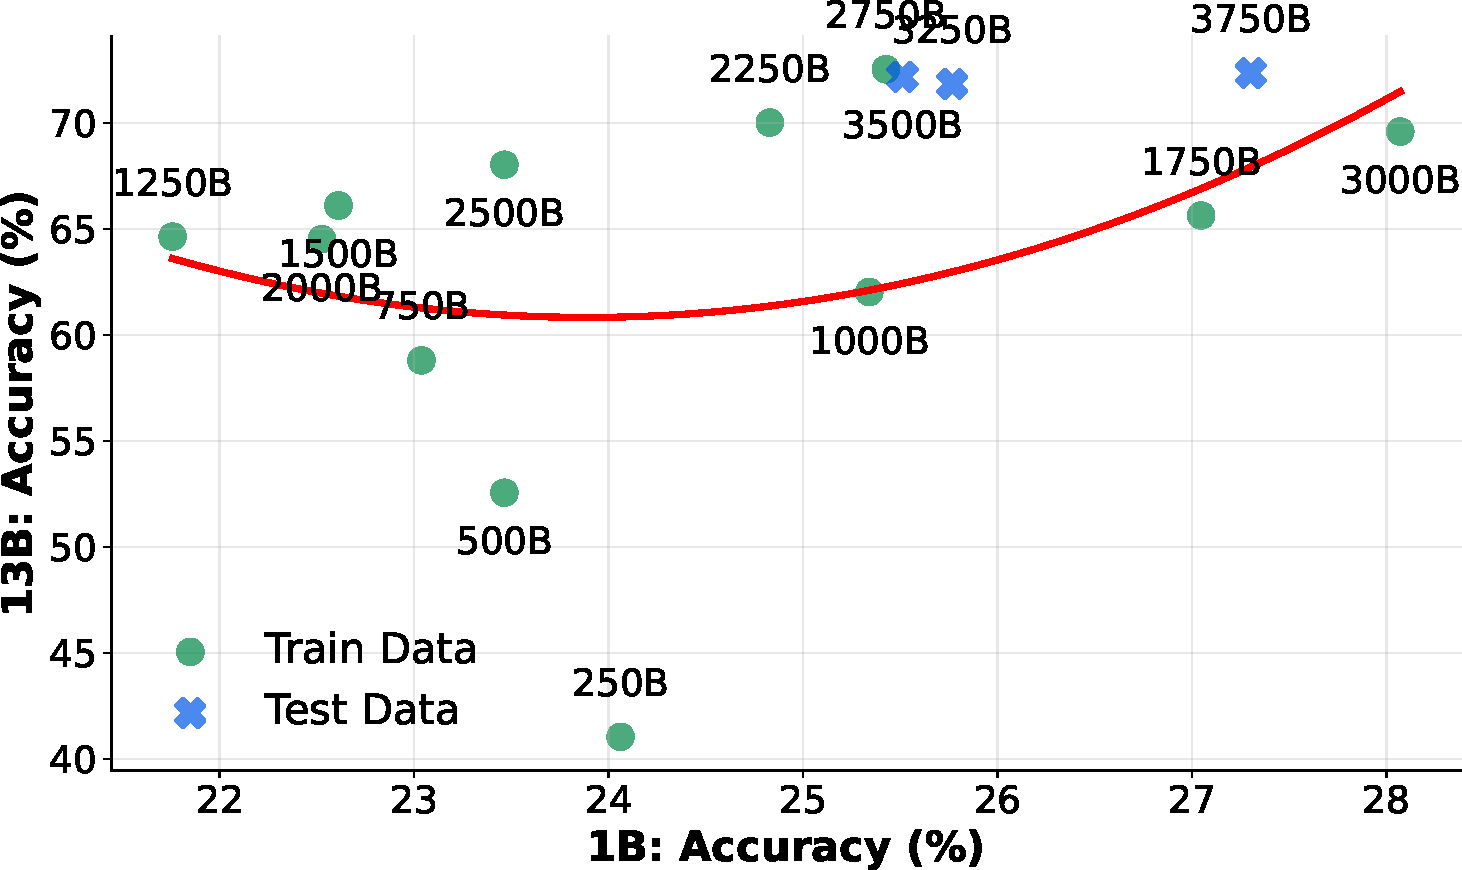
\includegraphics[width=\textwidth]{figs/arc-c_acc.pdf}
        \caption{Target metric Acc. as the proxy metric at 1B on ARC-C.}
    \end{subfigure}
    \hfill
    \begin{subfigure}[b]{0.497\textwidth}
        \centering
        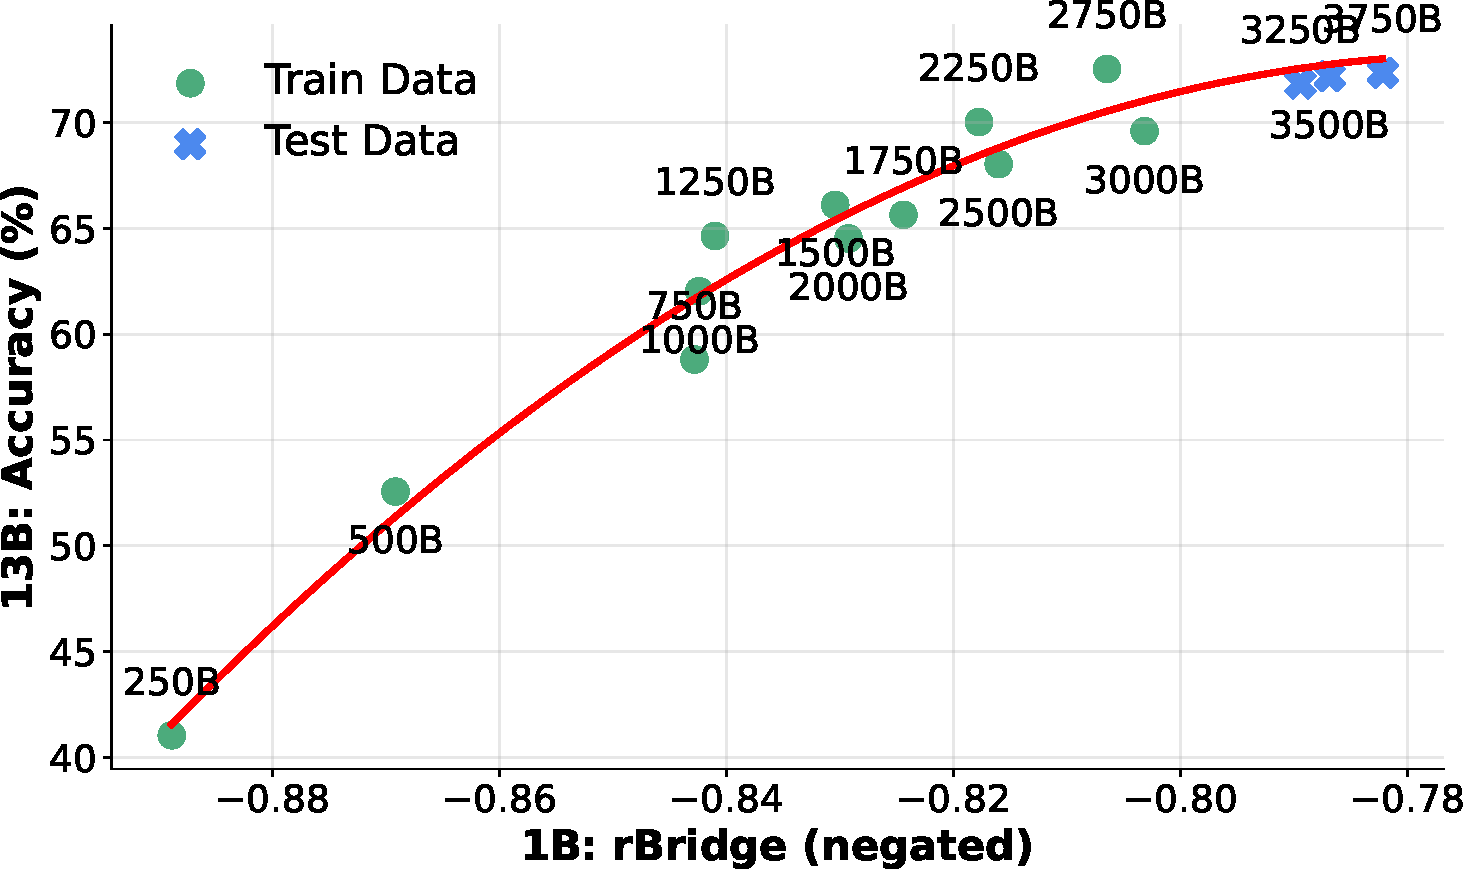
\includegraphics[width=\textwidth]{figs/arc-c_rbridge.pdf}
        \caption{\tsc{rBridge} as the proxy metric at 1B on ARC-C.\\~\\}
    \end{subfigure}

    \begin{subfigure}[b]{0.497\textwidth}
        \centering
        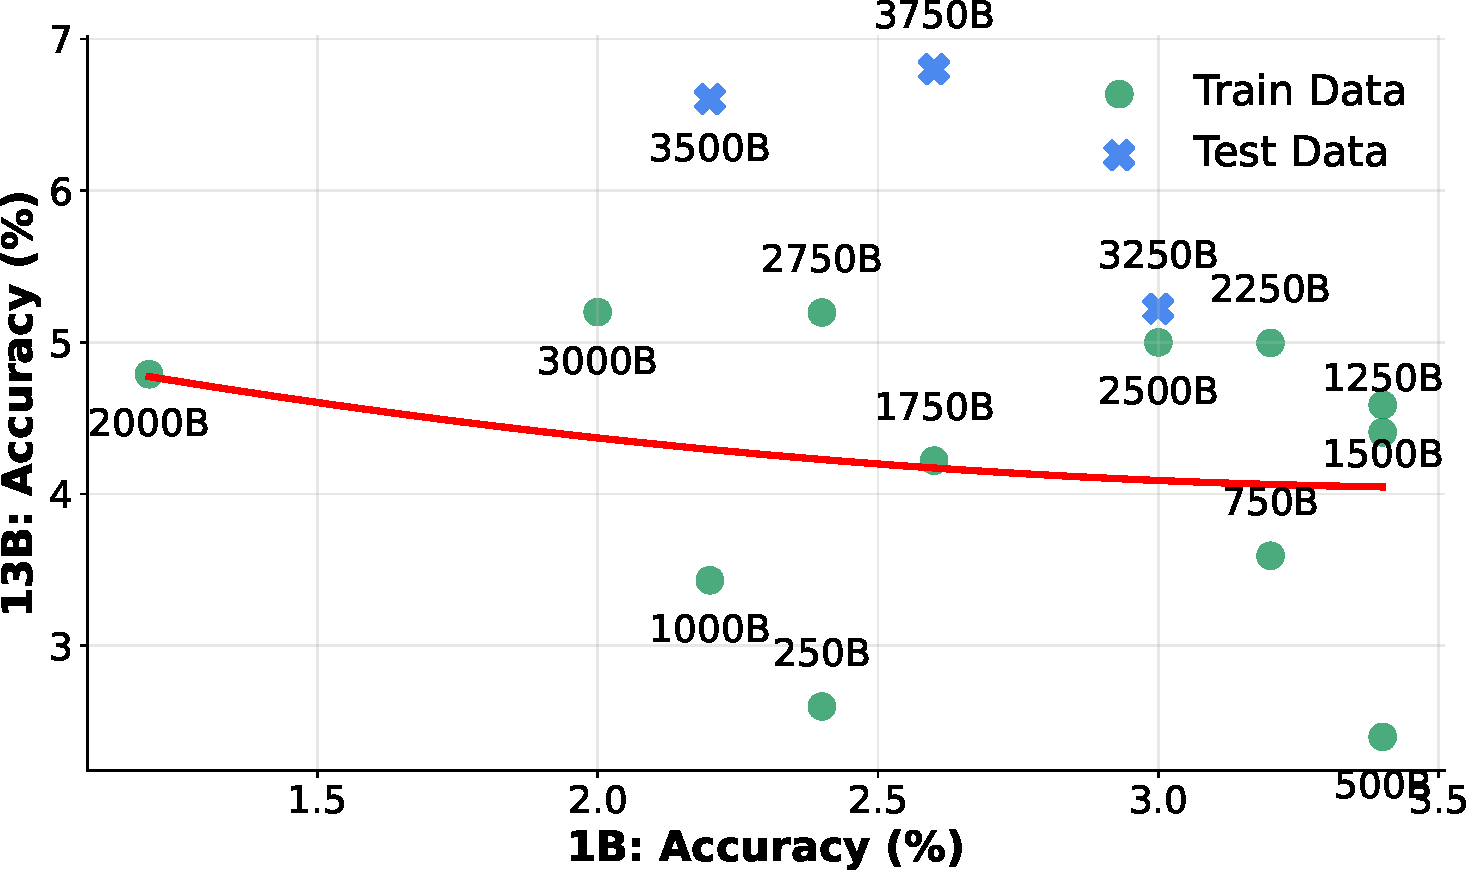
\includegraphics[width=\textwidth]{figs/math500_acc.pdf}
        \caption{Target metric Acc. as the proxy metric at 1B on MATH500.}
    \end{subfigure}
    \hfill
    \begin{subfigure}[b]{0.497\textwidth}
        \centering
        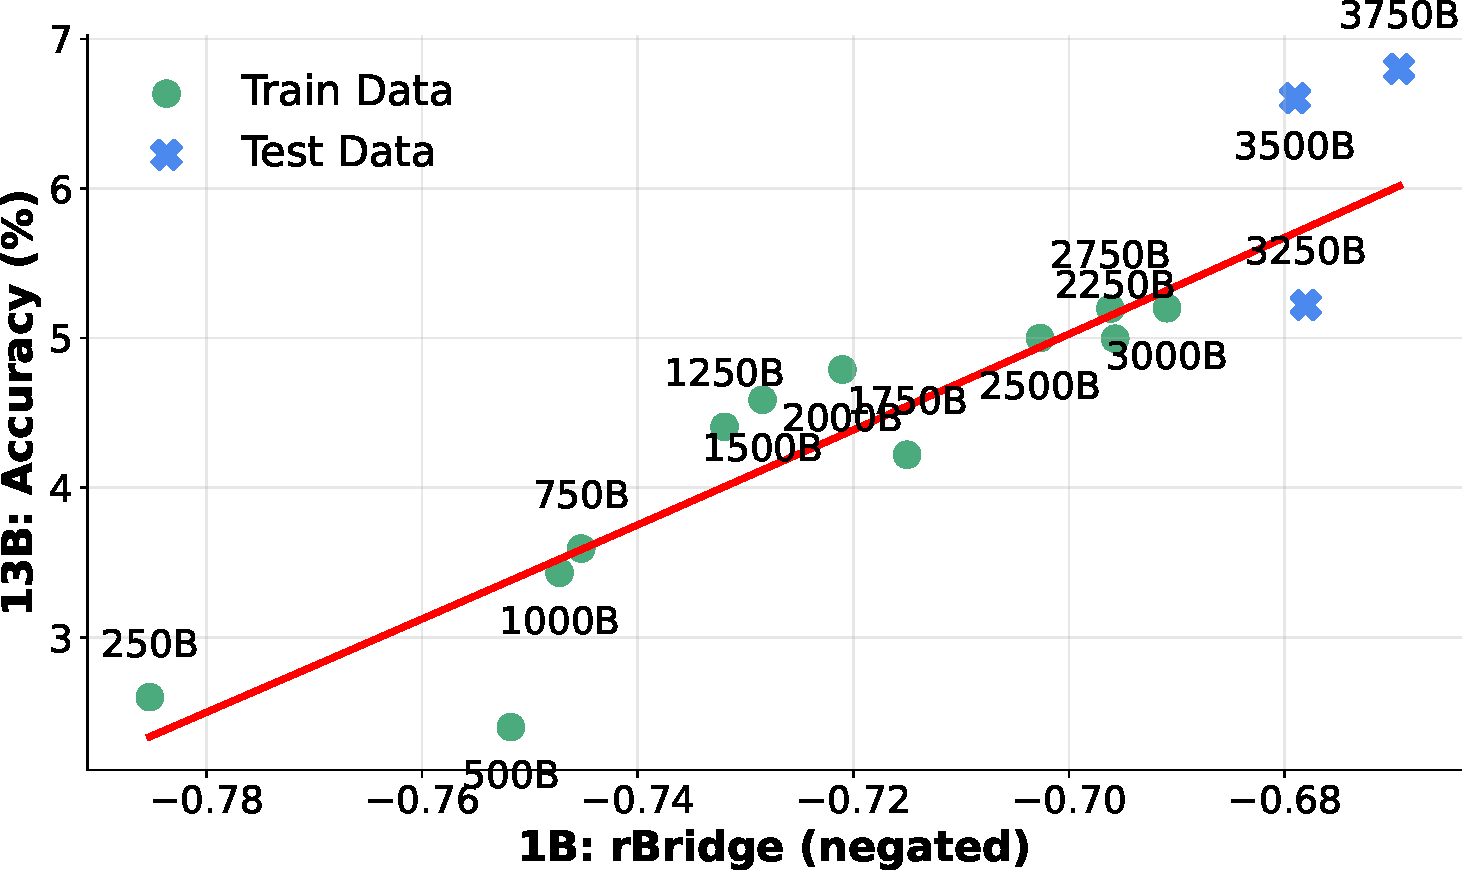
\includegraphics[width=\textwidth]{figs/math500_rbridge.pdf}
        \caption{\tsc{rBridge} as the proxy metric at 1B on MATH500.\\~\\}
    \end{subfigure}

        \begin{subfigure}[b]{0.497\textwidth}
        \centering
        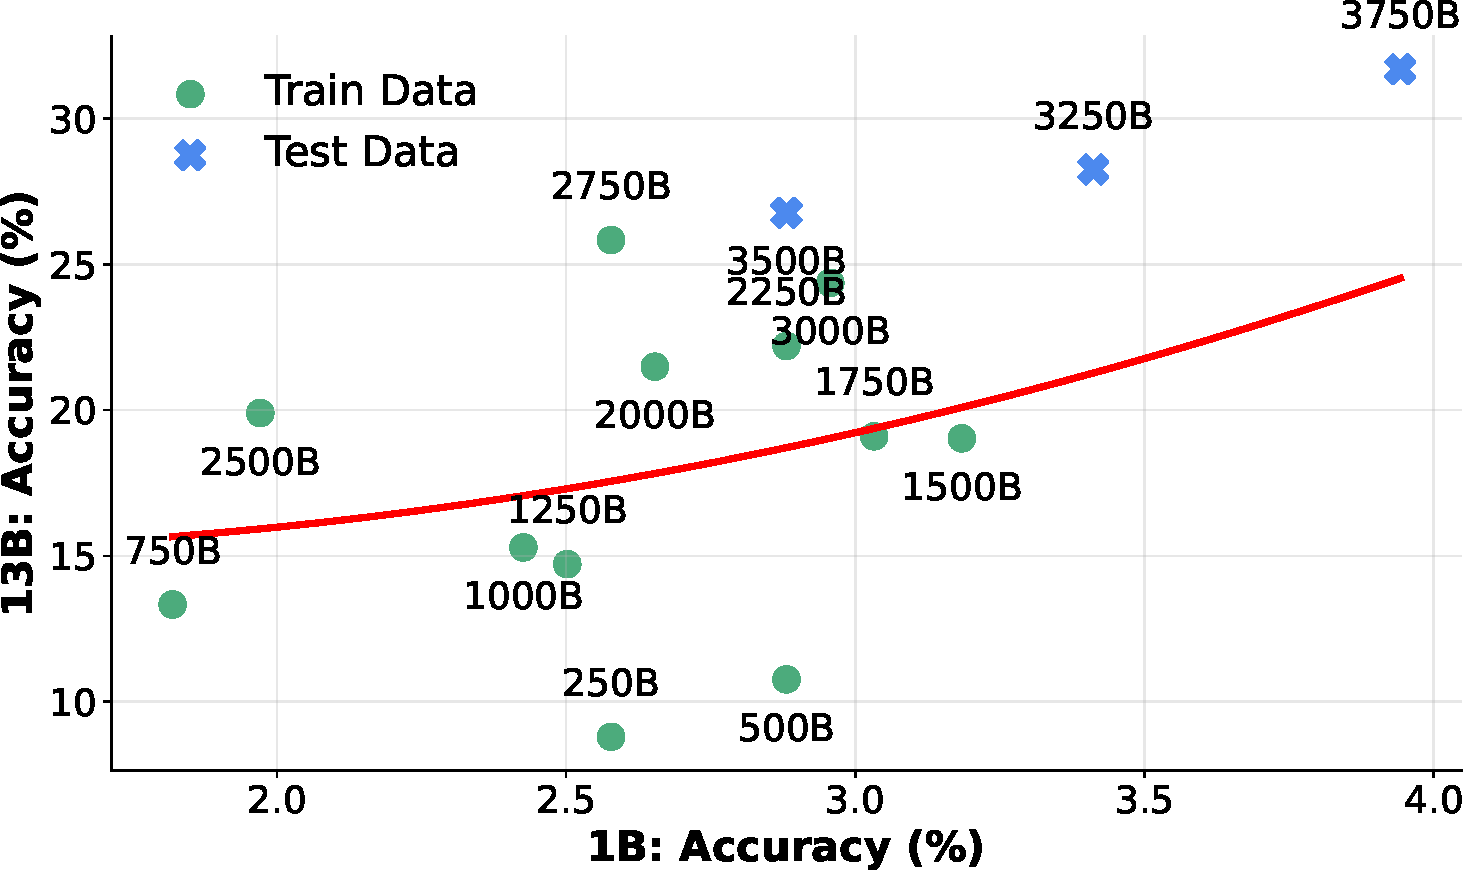
\includegraphics[width=\textwidth]{figs/gsm8k_acc.pdf}
        \caption{Target metric Acc. as the proxy metric at 1B on GSM8K.}
    \end{subfigure}
    \hfill
    \begin{subfigure}[b]{0.497\textwidth}
        \centering
        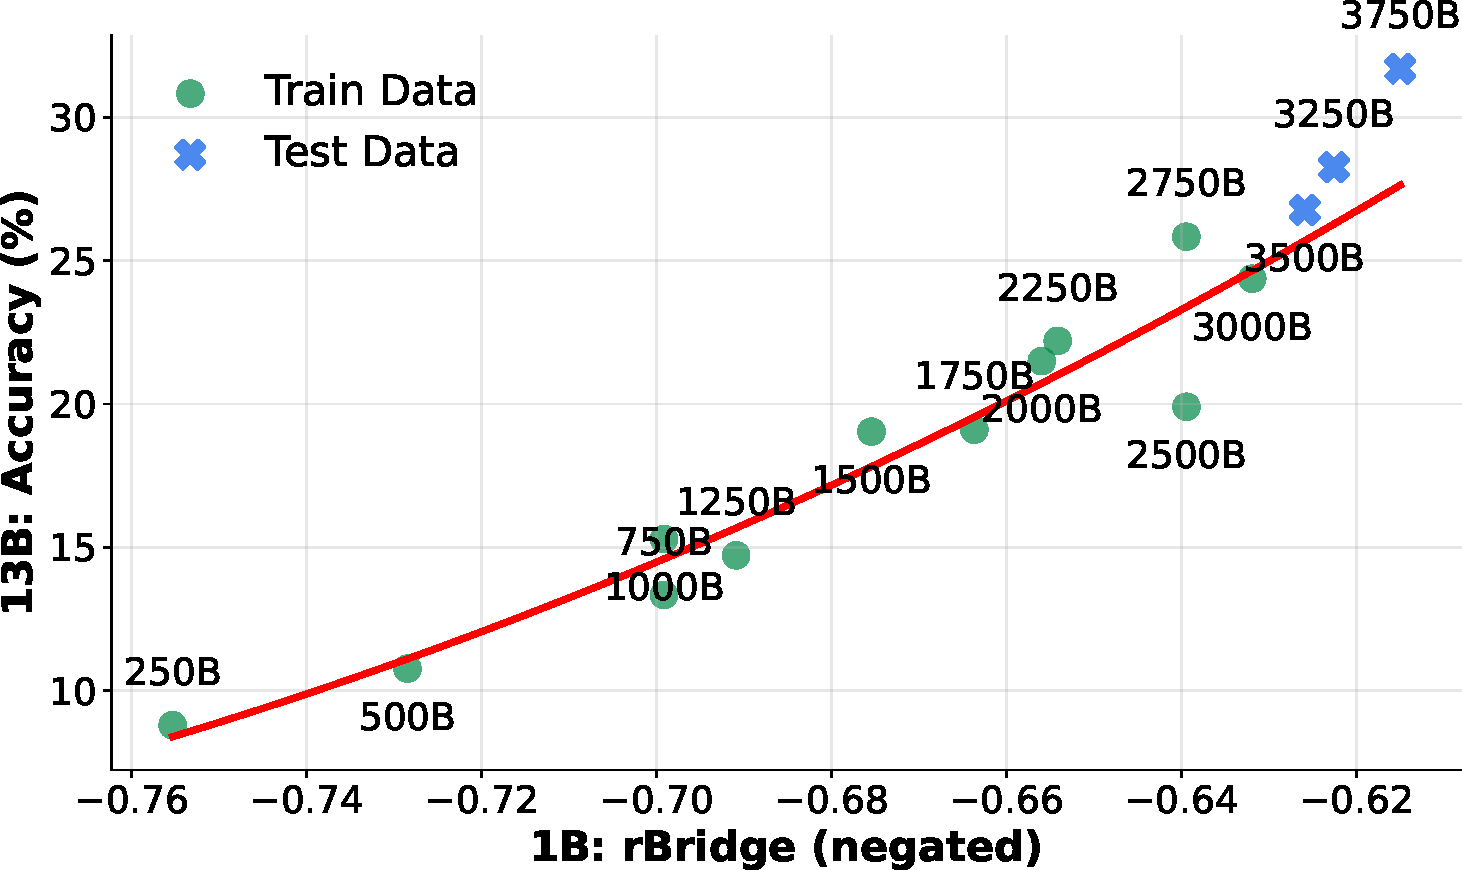
\includegraphics[width=\textwidth]{figs/gsm8k_rbridge.pdf}
        \caption{\tsc{rBridge} as the proxy metric at 1B on GSM8K.\\~\\}
    \end{subfigure}

    \caption{Example visualization from a fold of proxy-target relationship study at 1B $\rightarrow$ 13B on CQA, ARC-C, MATH500, and GSM8K. Each data point represents equal trained tokens for the proxy and target model.}
    \label{fig:curve_fit}
\end{figure}

\begin{figure}[tb!]
    \centering
            \begin{subfigure}[b]{0.497\textwidth}
        \centering
        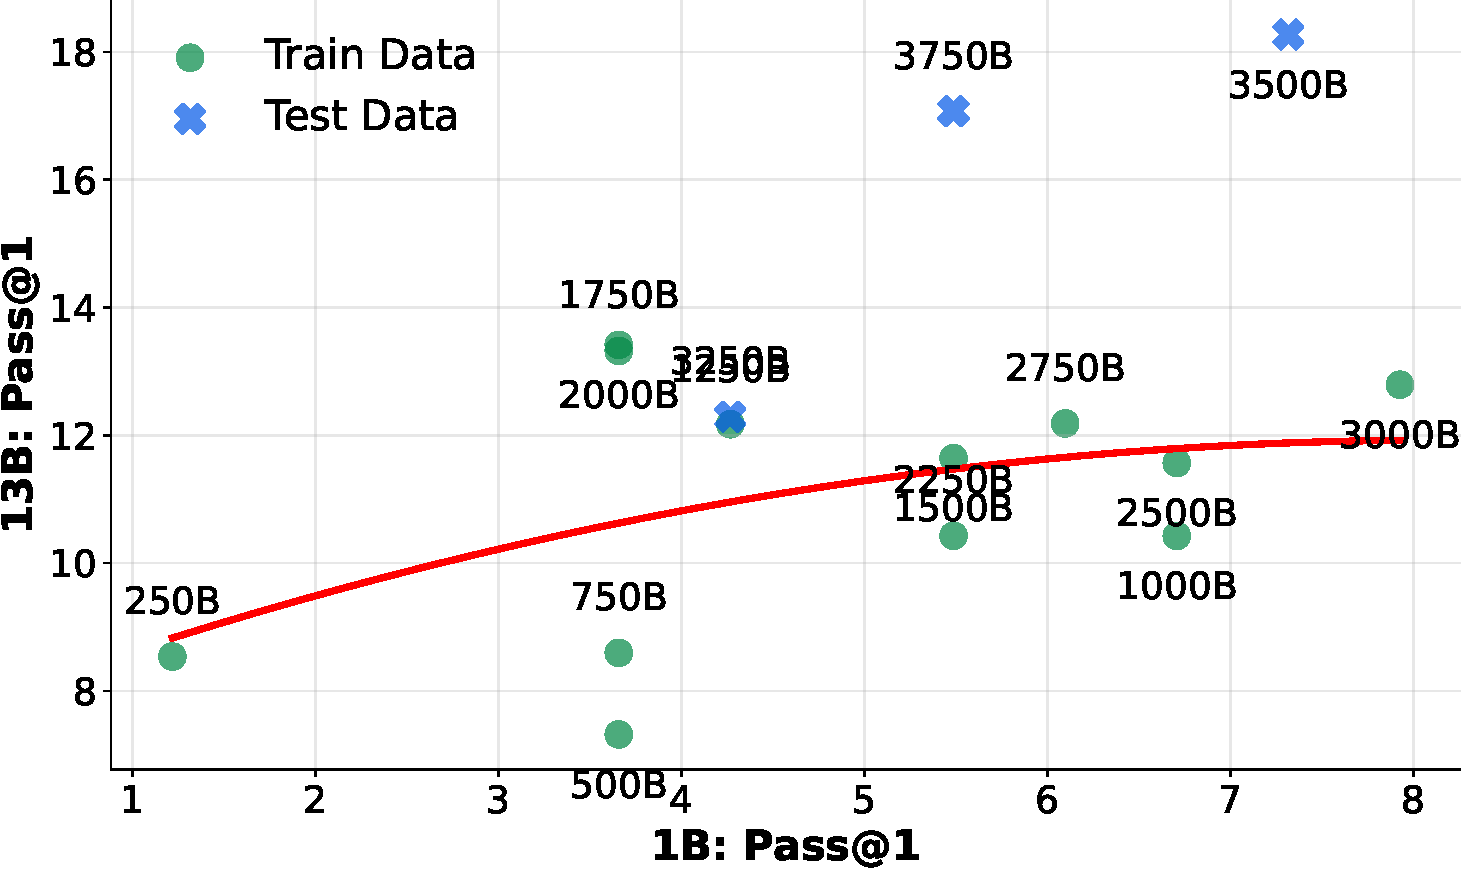
\includegraphics[width=\textwidth]{figs/humaneval_pass_1.pdf}
        \caption{Target metric Acc. as the proxy metric at 1B.}
    \end{subfigure}
    \hfill
    \begin{subfigure}[b]{0.497\textwidth}
        \centering
        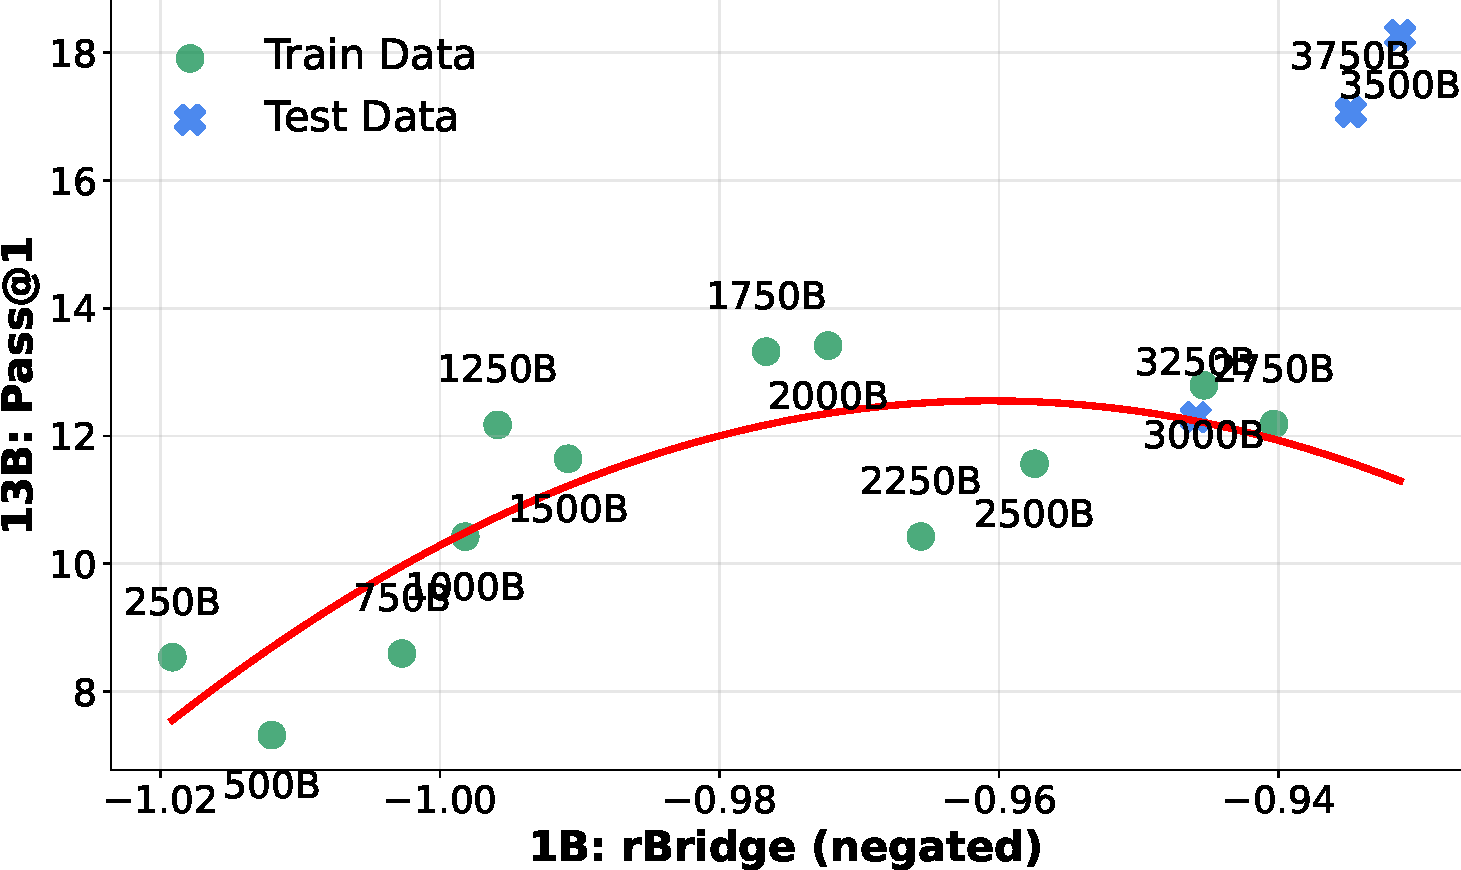
\includegraphics[width=\textwidth]{figs/humaneval_rbridge.pdf}
        \caption{\tsc{rBridge} as the proxy metric at 1B.}
    \end{subfigure}
    
    \caption{Example visualization from a fold of proxy-target relationship study at 1B $\rightarrow$ 13B on HumanEval. Each data point represents equal trained tokens for the proxy and target model.}
    \label{fig:curve_fit_1}
\end{figure}


\begin{table*}[htbp]
\centering
\resizebox{\textwidth}{!}{
\begin{tabular}{llcccccc>{\columncolor{gray!15}}c}
\toprule
\textbf{Benchmark} & \textbf{Method:} & \textbf{Acc./p@1} & \textbf{iSFT} & \textbf{TED} & \textbf{MPCA} & \textbf{NLL} & \textbf{$R^\phi$} & \textbf{\texttt{rBridge}} \\
\midrule
\multirow{2}{*}{GSM8K} & Train R$^2$ & 0.363 & 0.385 & 0.565 & 0.129 & 0.868 & \underline{0.951} & \textbf{0.956} \\
 & Test MAE & 5.807 & 5.536 & 7.054 & 79.761 & 3.302 & \underline{1.715} & \textbf{1.616} \\
\midrule
\multirow{2}{*}{MATH500} & Train R$^2$ & 0.088 & 0.128 & 0.199 & 0.182 & \textbf{0.557} & 0.544 & \underline{0.555} \\
 & Test MAE & 1.178 & 0.888 & 0.805 & 0.849 & 0.692 & \underline{0.609} & \textbf{0.605} \\
\midrule
\multirow{2}{*}{ARC-C} & Train R$^2$ & 0.187 & 0.153 & 0.522 & 0.331 & 0.160 & \underline{0.938} & \textbf{0.964} \\
 & Test MAE & 6.921 & 8.317 & 6.248 & 22.685 & 6.679 & \underline{1.590} & \textbf{1.279} \\
\midrule
\multirow{2}{*}{CQA} & Train R$^2$ & 0.677 & 0.543 & 0.783 & 0.385 & 0.068 & \underline{0.845} & \textbf{0.910} \\
 & Test MAE & 3.593 & 6.264 & 2.837 & 4.952 & 5.055 & \underline{2.283} & \textbf{1.715} \\
\midrule
\multicolumn{2}{l}{\textbf{Average Train R$^2$ ($\uparrow$)}} & 0.329 & 0.302 & 0.517 & 0.257 & 0.413 & \underline{0.820} & \textbf{0.846} \\
\multicolumn{2}{l}{\textbf{Average Test MAE ($\downarrow$)}} & 4.375 & 5.251 & 4.236 & 27.062 & 3.932 & \underline{1.549} & \textbf{1.304} \\
\bottomrule
\end{tabular}}
\caption{Detailed results of 1B $\rightarrow$ 13B+SFT (Pre-to-Post). Train fitting and test is done using 5-fold cross validation (\textbf{\S\ \ref{sec:protocol}}). Best value across methods is \textbf{bolded}, and second best is \underline{underlined}.}
\label{tab:olmo_1b_13b_pre_to_post}
\end{table*}

\begin{table*}[htbp]
\centering
\resizebox{\textwidth}{!}{
\begin{tabular}{llcccccc>{\columncolor{gray!15}}c}
\toprule
\textbf{Benchmark} & \textbf{Method:} & \textbf{Acc./p@1} & \textbf{iSFT} & \textbf{TED} & \textbf{MPCA} & \textbf{NLL} & \textbf{$R^\phi$} & \textbf{\texttt{rBridge}} \\
\midrule
\multirow{2}{*}{GSM8K} & Train R$^2$ & 0.281 & 0.398 & 0.706 & 0.076 & \underline{0.814} & \textbf{0.972} & \textbf{0.972} \\
 & Test MAE & 7.755 & 7.299 & 6.505 & 107.493 & 6.935 & \underline{1.676} & \textbf{1.601} \\
\midrule
\multirow{2}{*}{MATH500} & Train R$^2$ & 0.193 & 0.196 & 0.166 & 0.019 & 0.823 & \underline{0.832} & \textbf{0.834} \\
 & Test MAE & 98.093 & 1.869 & 1.985 & 6.907 & 0.815 & \underline{0.739} & \textbf{0.718} \\
\midrule
\multirow{2}{*}{ARC-C} & Train R$^2$ & 0.206 & 0.169 & 0.582 & 0.346 & 0.144 & \underline{0.926} & \textbf{0.949} \\
 & Test MAE & 4.734 & 5.976 & 4.491 & 7.588 & 4.985 & \underline{1.560} & \textbf{1.384} \\
\midrule
\multirow{2}{*}{\makecell{MMLU Pro\\(STEM)}} & Train R$^2$ & 0.057 & --- & 0.031 & 0.210 & \underline{0.344} & \textbf{0.756} & \textbf{0.756} \\
 & Test MAE & 2.075 & --- & 1.930 & \underline{1.864} & 2.133 & \textbf{1.326} & \textbf{1.326} \\
\midrule
\multirow{2}{*}{CQA} & Train R$^2$ & 0.624 & 0.634 & 0.528 & 0.332 & 0.046 & \underline{0.765} & \textbf{0.766} \\
 & Test MAE & 4.105 & 5.516 & 3.630 & 4.199 & 3.664 & \textbf{2.382} & \underline{2.384} \\
\midrule
\multirow{2}{*}{HumanEval} & Train R$^2$ & 0.514 & --- & 0.101 & 0.245 & \textbf{0.759} & 0.666 & \underline{0.679} \\
 & Test MAE & 1.946 & --- & 2.733 & 2.947 & \textbf{1.424} & 1.555 & \underline{1.474} \\
\midrule
\multicolumn{2}{l}{\textbf{Average Train R$^2$ ($\uparrow$)}} & 0.312 & 0.349 & 0.352 & 0.205 & 0.488 & \underline{0.820} & \textbf{0.826} \\
\multicolumn{2}{l}{\textbf{Average Test MAE ($\downarrow$)}} & 19.785 & 5.165 & 3.546 & 21.833 & 3.276 & \underline{1.540} & \textbf{1.481} \\
\bottomrule
\end{tabular}}
\caption{Detailed results of 1B $\rightarrow$ 32B (Pre-to-Pre). Train fitting and test is done using 5-fold cross validation (\textbf{\S\ \ref{sec:protocol}}). Best value across methods is \textbf{bolded}, and second best is \underline{underlined}.}
\label{tab:olmo_1b_32b_pre_to_pre}
\end{table*}

\begin{figure}[tb]
    \centering
    \begin{subfigure}[b]{0.497\textwidth}
        \centering
        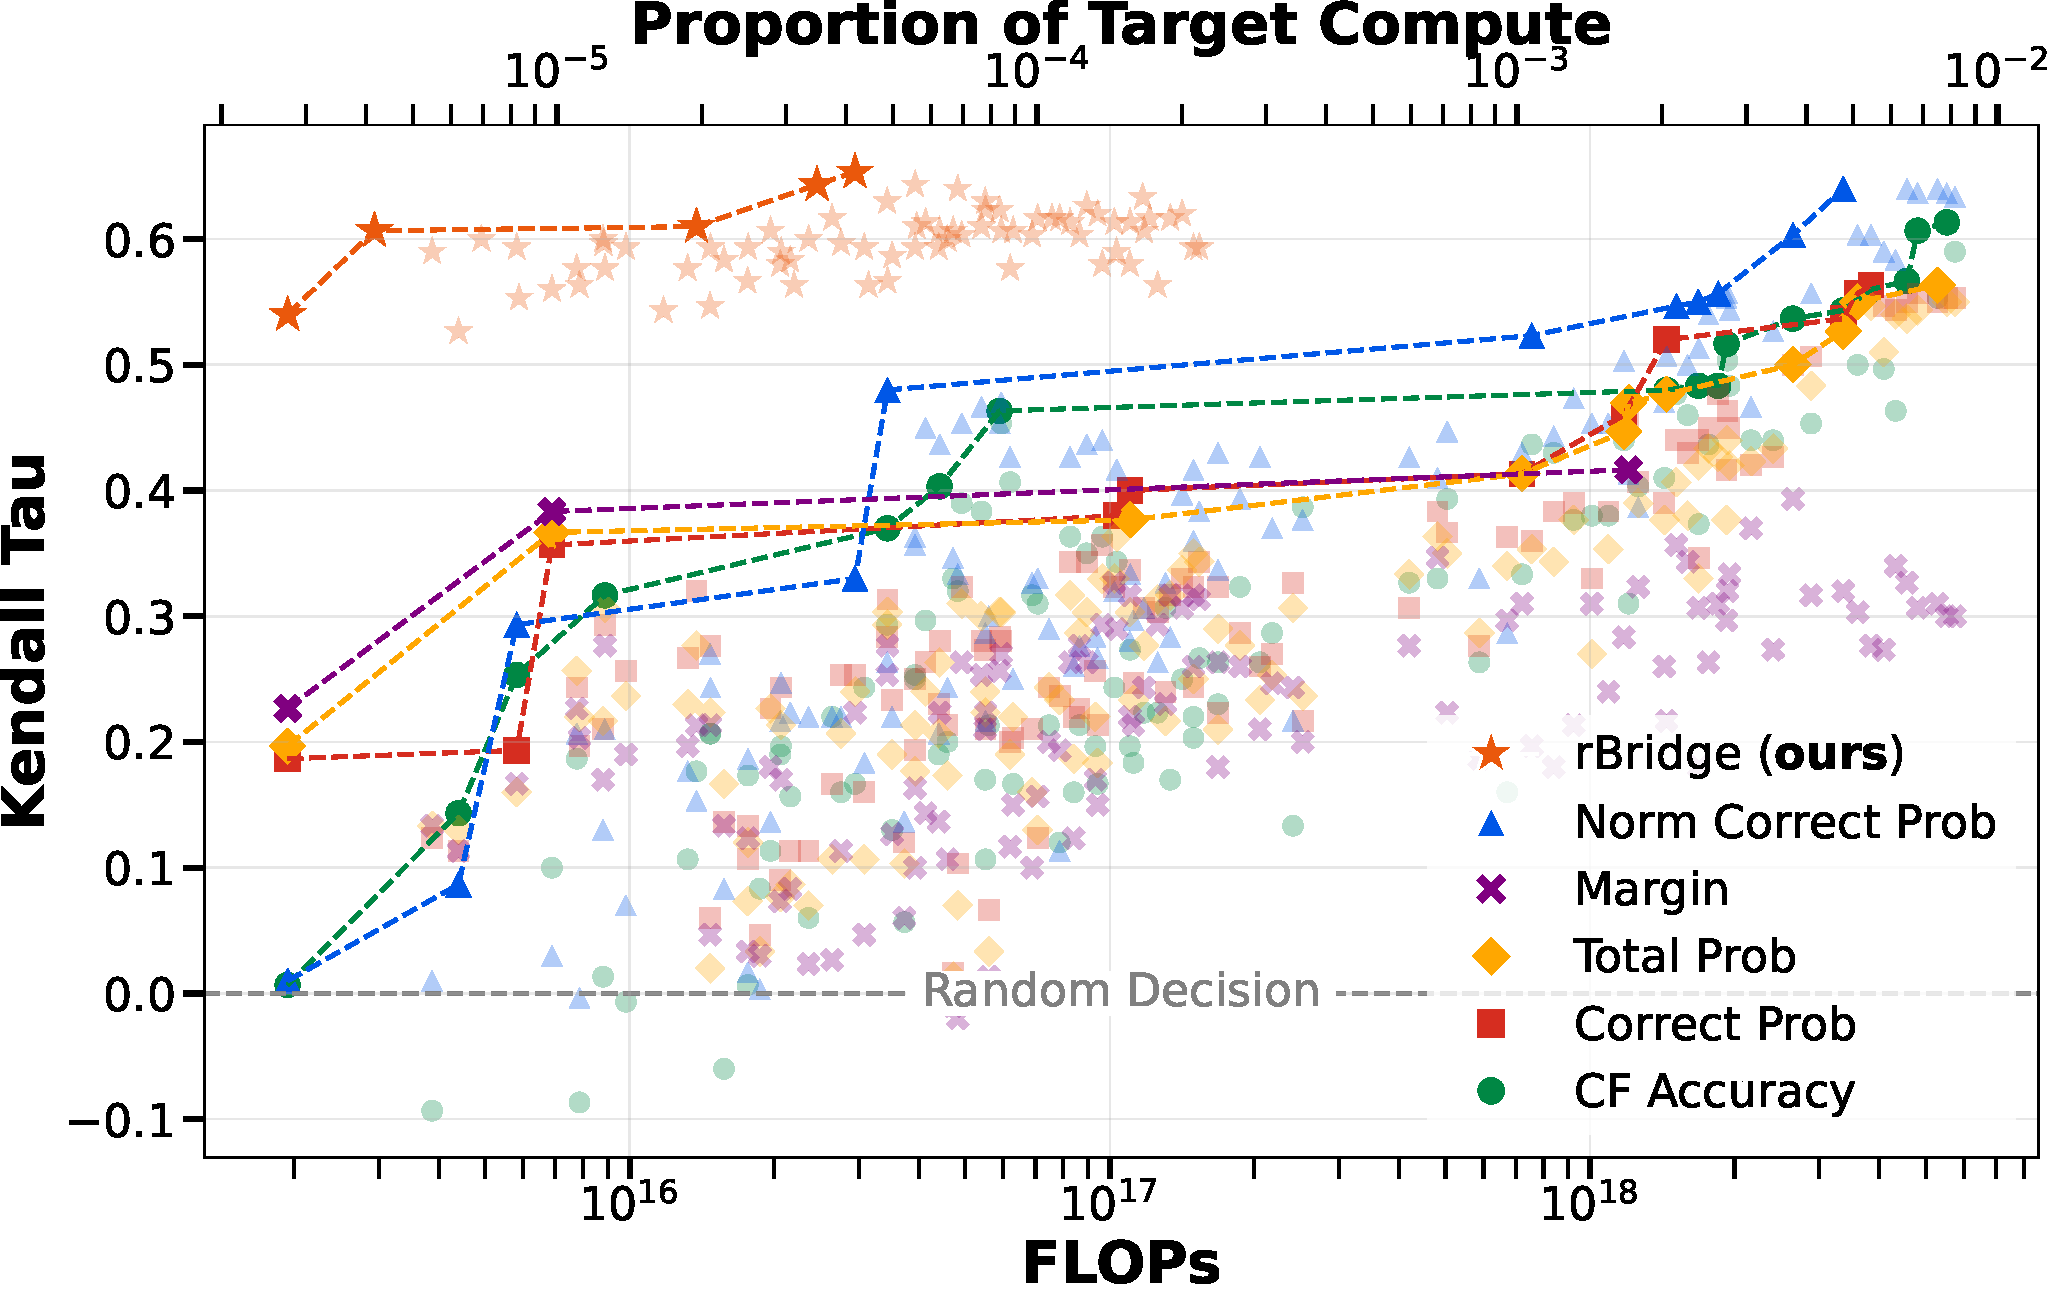
\includegraphics[width=\textwidth]{figs/pareto_kendall.pdf}
        \caption{Kendal Tau results across 3.7 - 97.9M proxy model size, and across intermediary checkpoints.}
        \label{fig:pareto_kendall}
    \end{subfigure}
    \hfill
    \begin{subfigure}[b]{0.497\textwidth}
        \centering
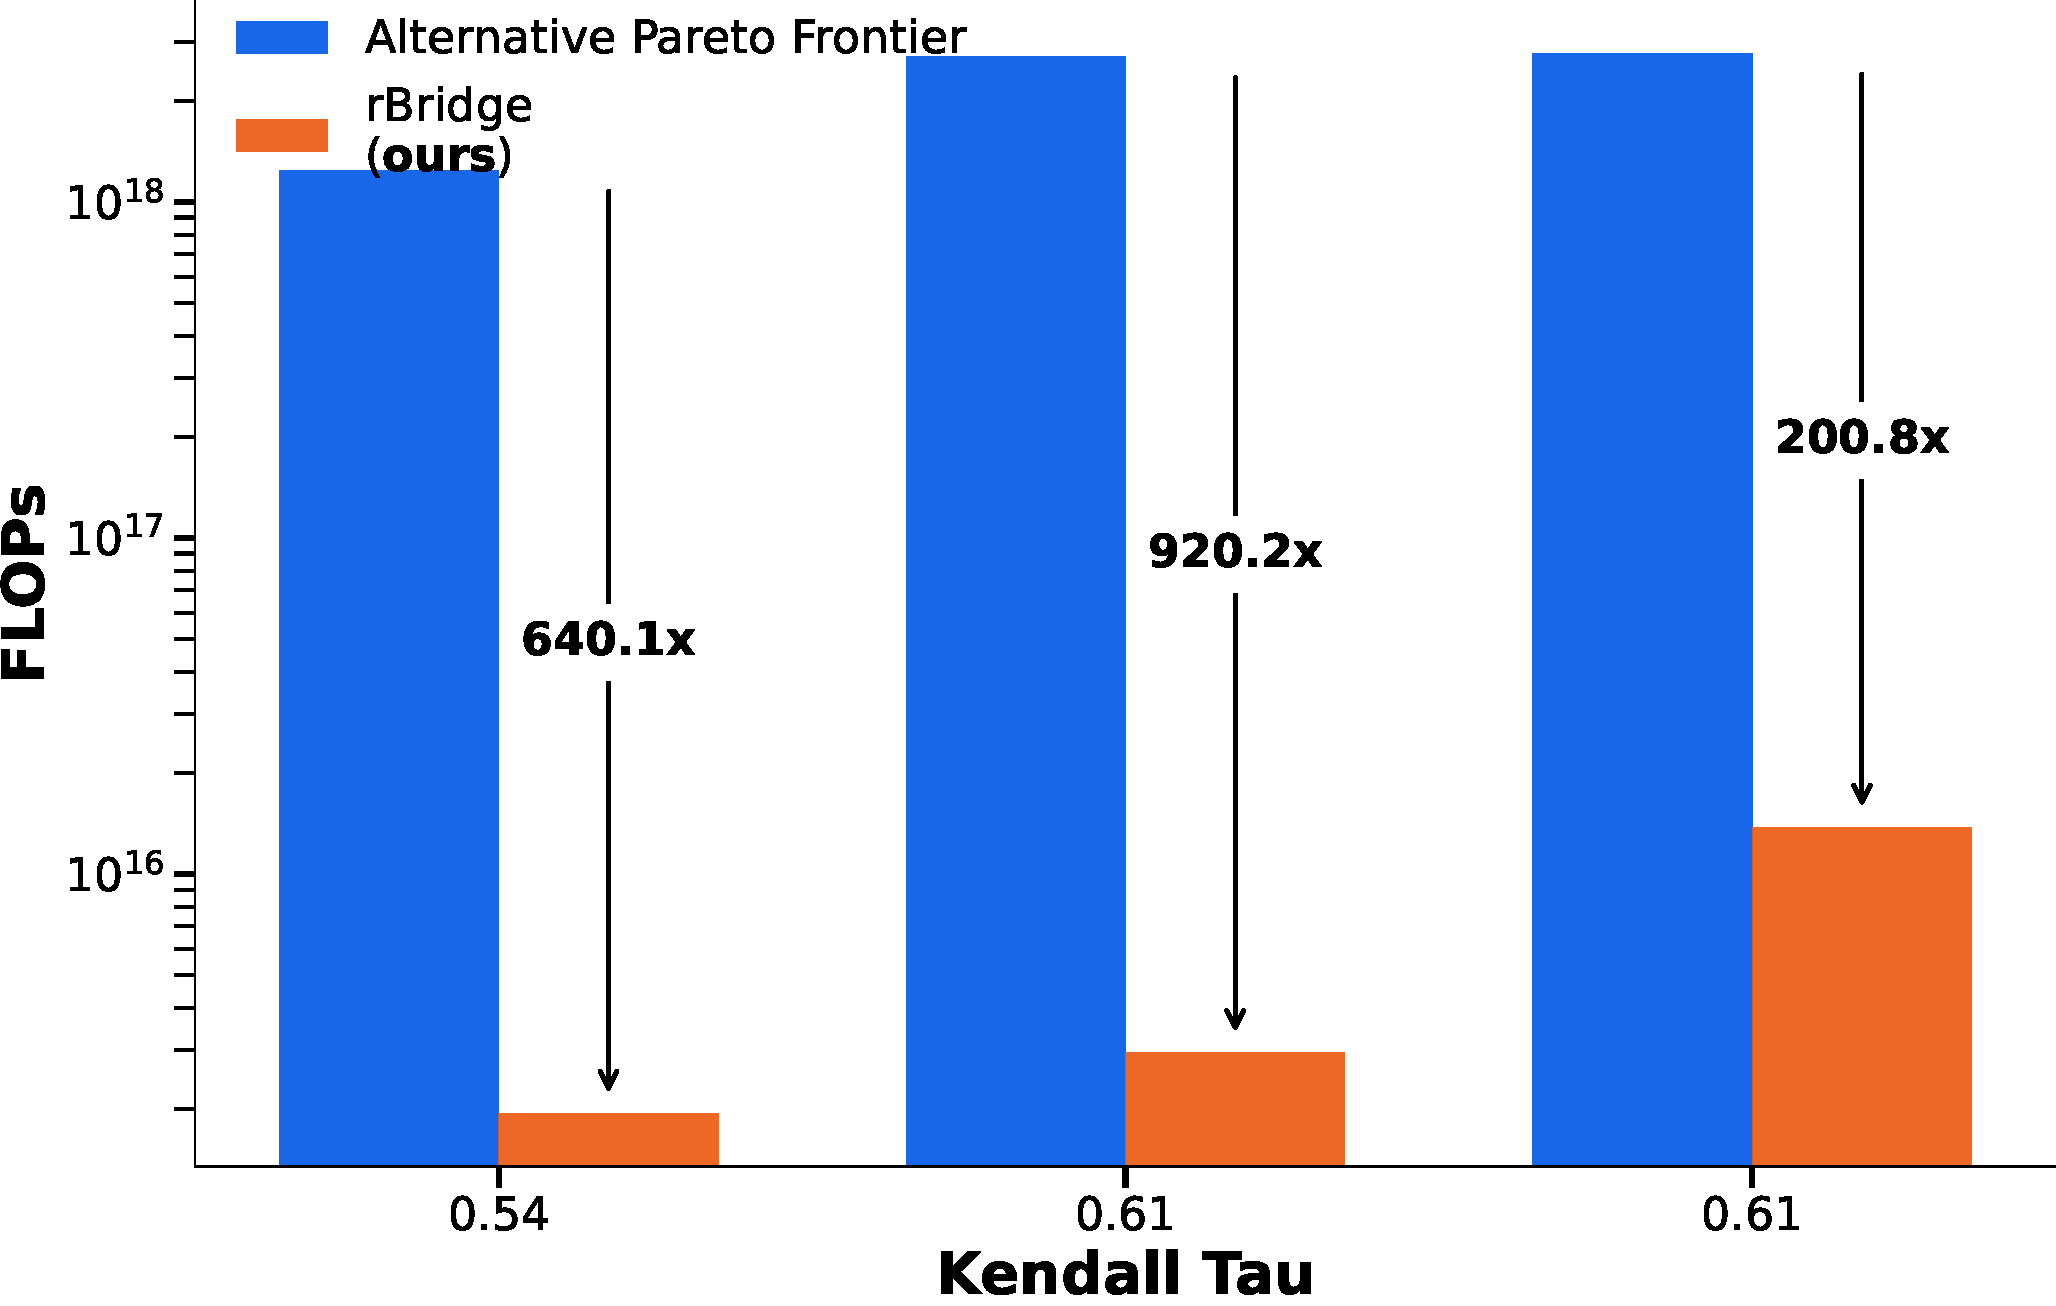
\includegraphics[width=\textwidth]{figs/flops_savings_kendall.pdf}
        \caption{\tsc{rBridge} saves FLOPs by a factor of 200.8$\times$ to 920.2$\times$.}
        \label{fig:flops_kendall}
    \end{subfigure}
    \caption{\tsc{rBridge} improves the pareto frontier in pre-training dataset ranking for 1.2B target model size. Values are averages aggregated across ARC-C and CQA. The two most compute efficient points in \tsc{rBridge}'s pareto frontier is (1) 3.7M model size trained on 87.3M tokens, and (2) 6M model size trained on 81.6M tokens.}
    \label{fig:kendall}
\end{figure}

\section{Proxy Benchmarks are Unreliable} \label{app:proxy_task}

Refer to Fig. \ref{fig:proxytask}.

\begin{figure}[htb]
    \centering
    \begin{subfigure}[b]{0.497\textwidth}
        \centering
        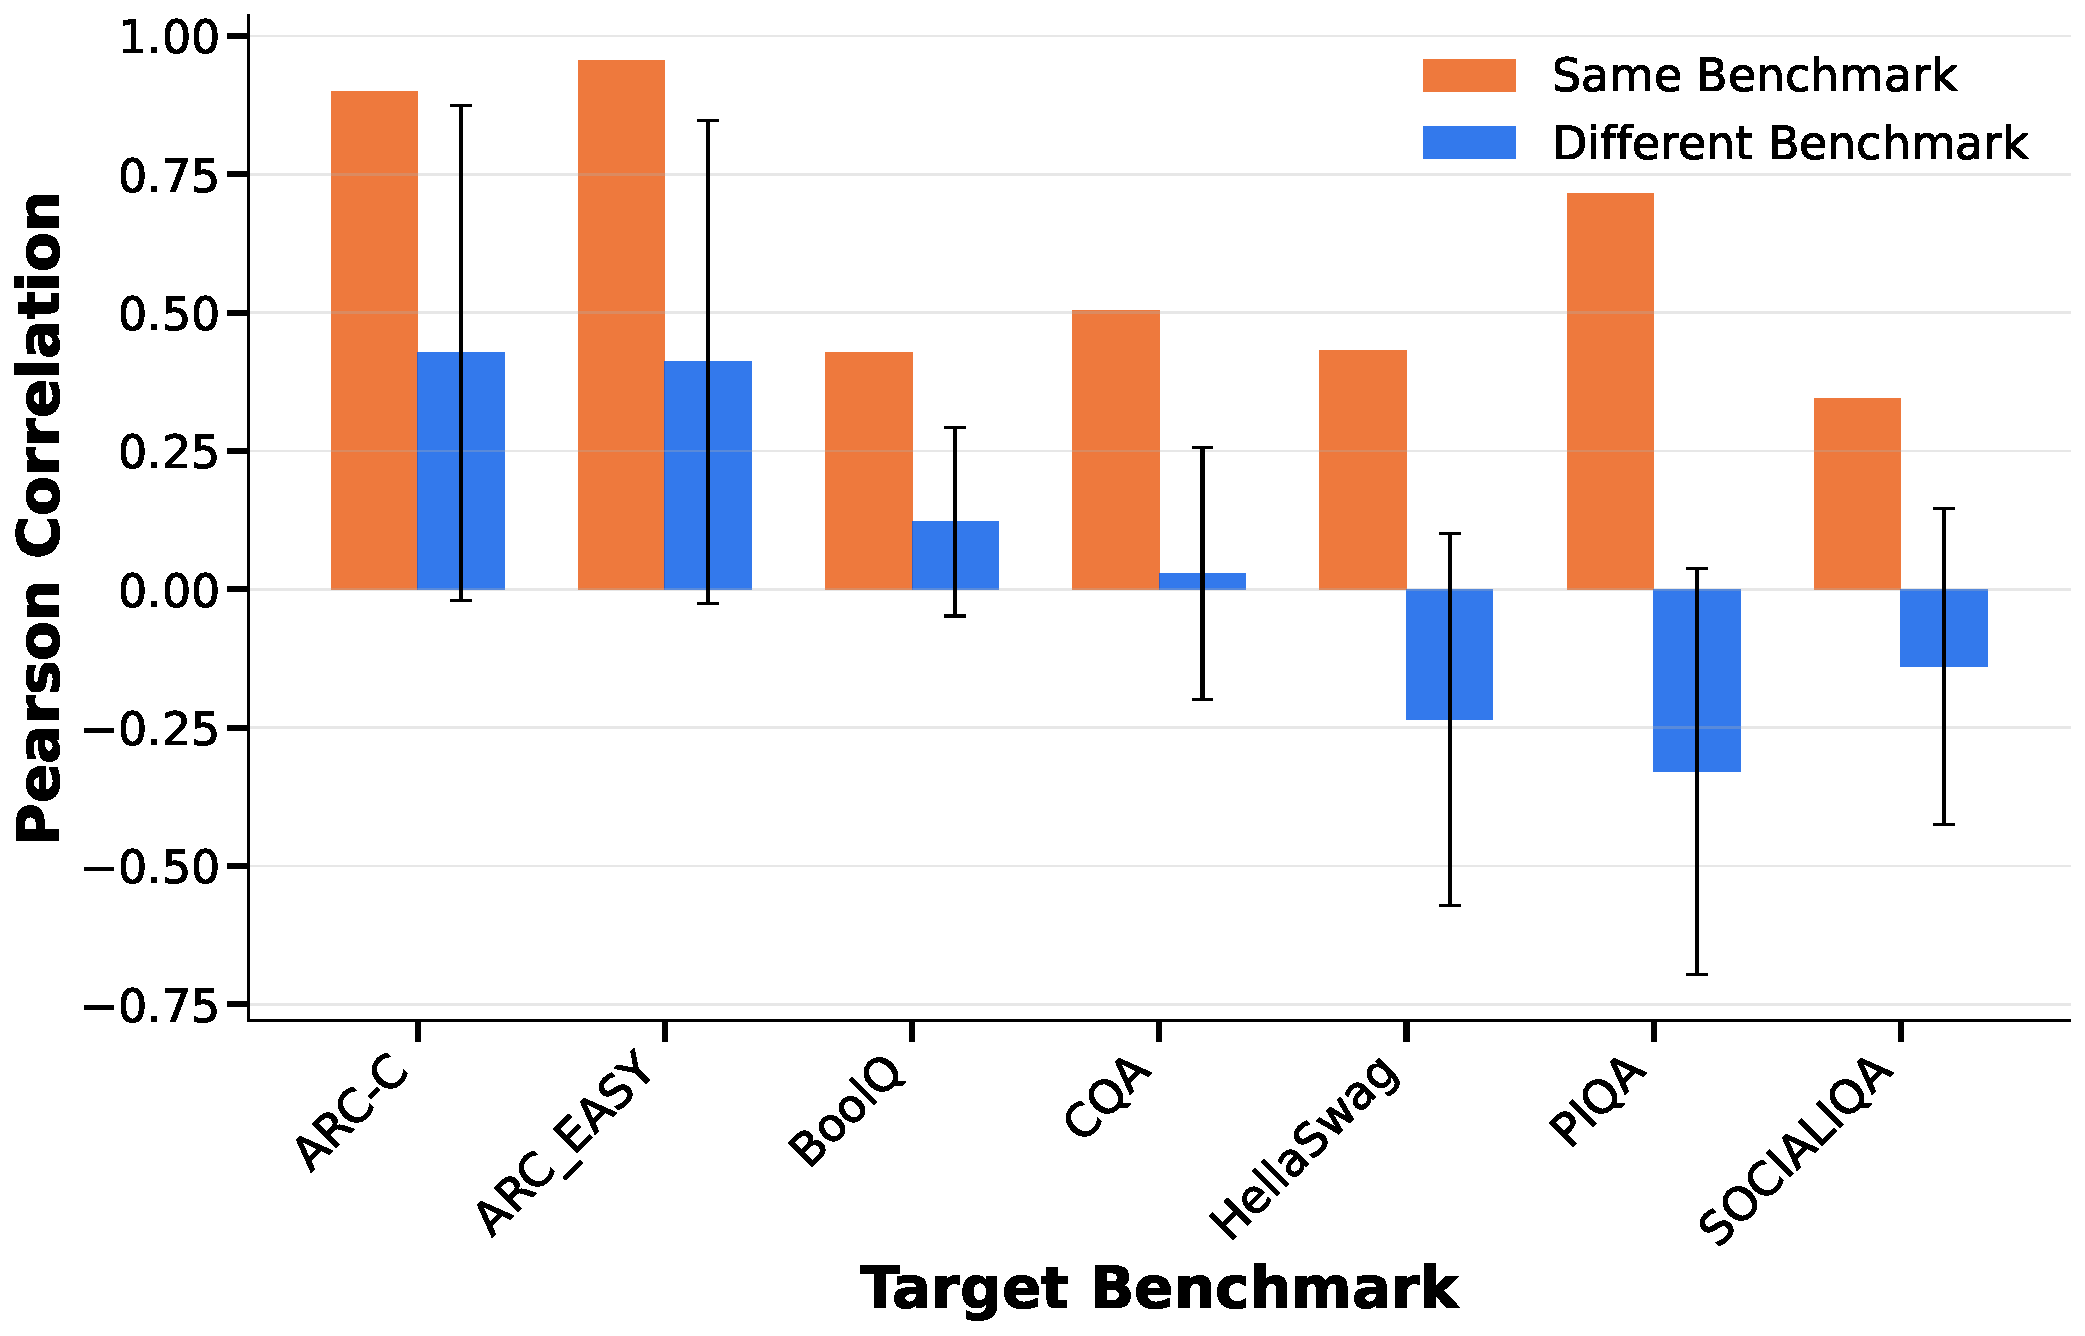
\includegraphics[width=\textwidth]{figs/benchmark_correlation.pdf}
        \label{fig:proxy_corr}
    \end{subfigure}
    \hfill
    \begin{subfigure}[b]{0.497\textwidth}
        \centering
        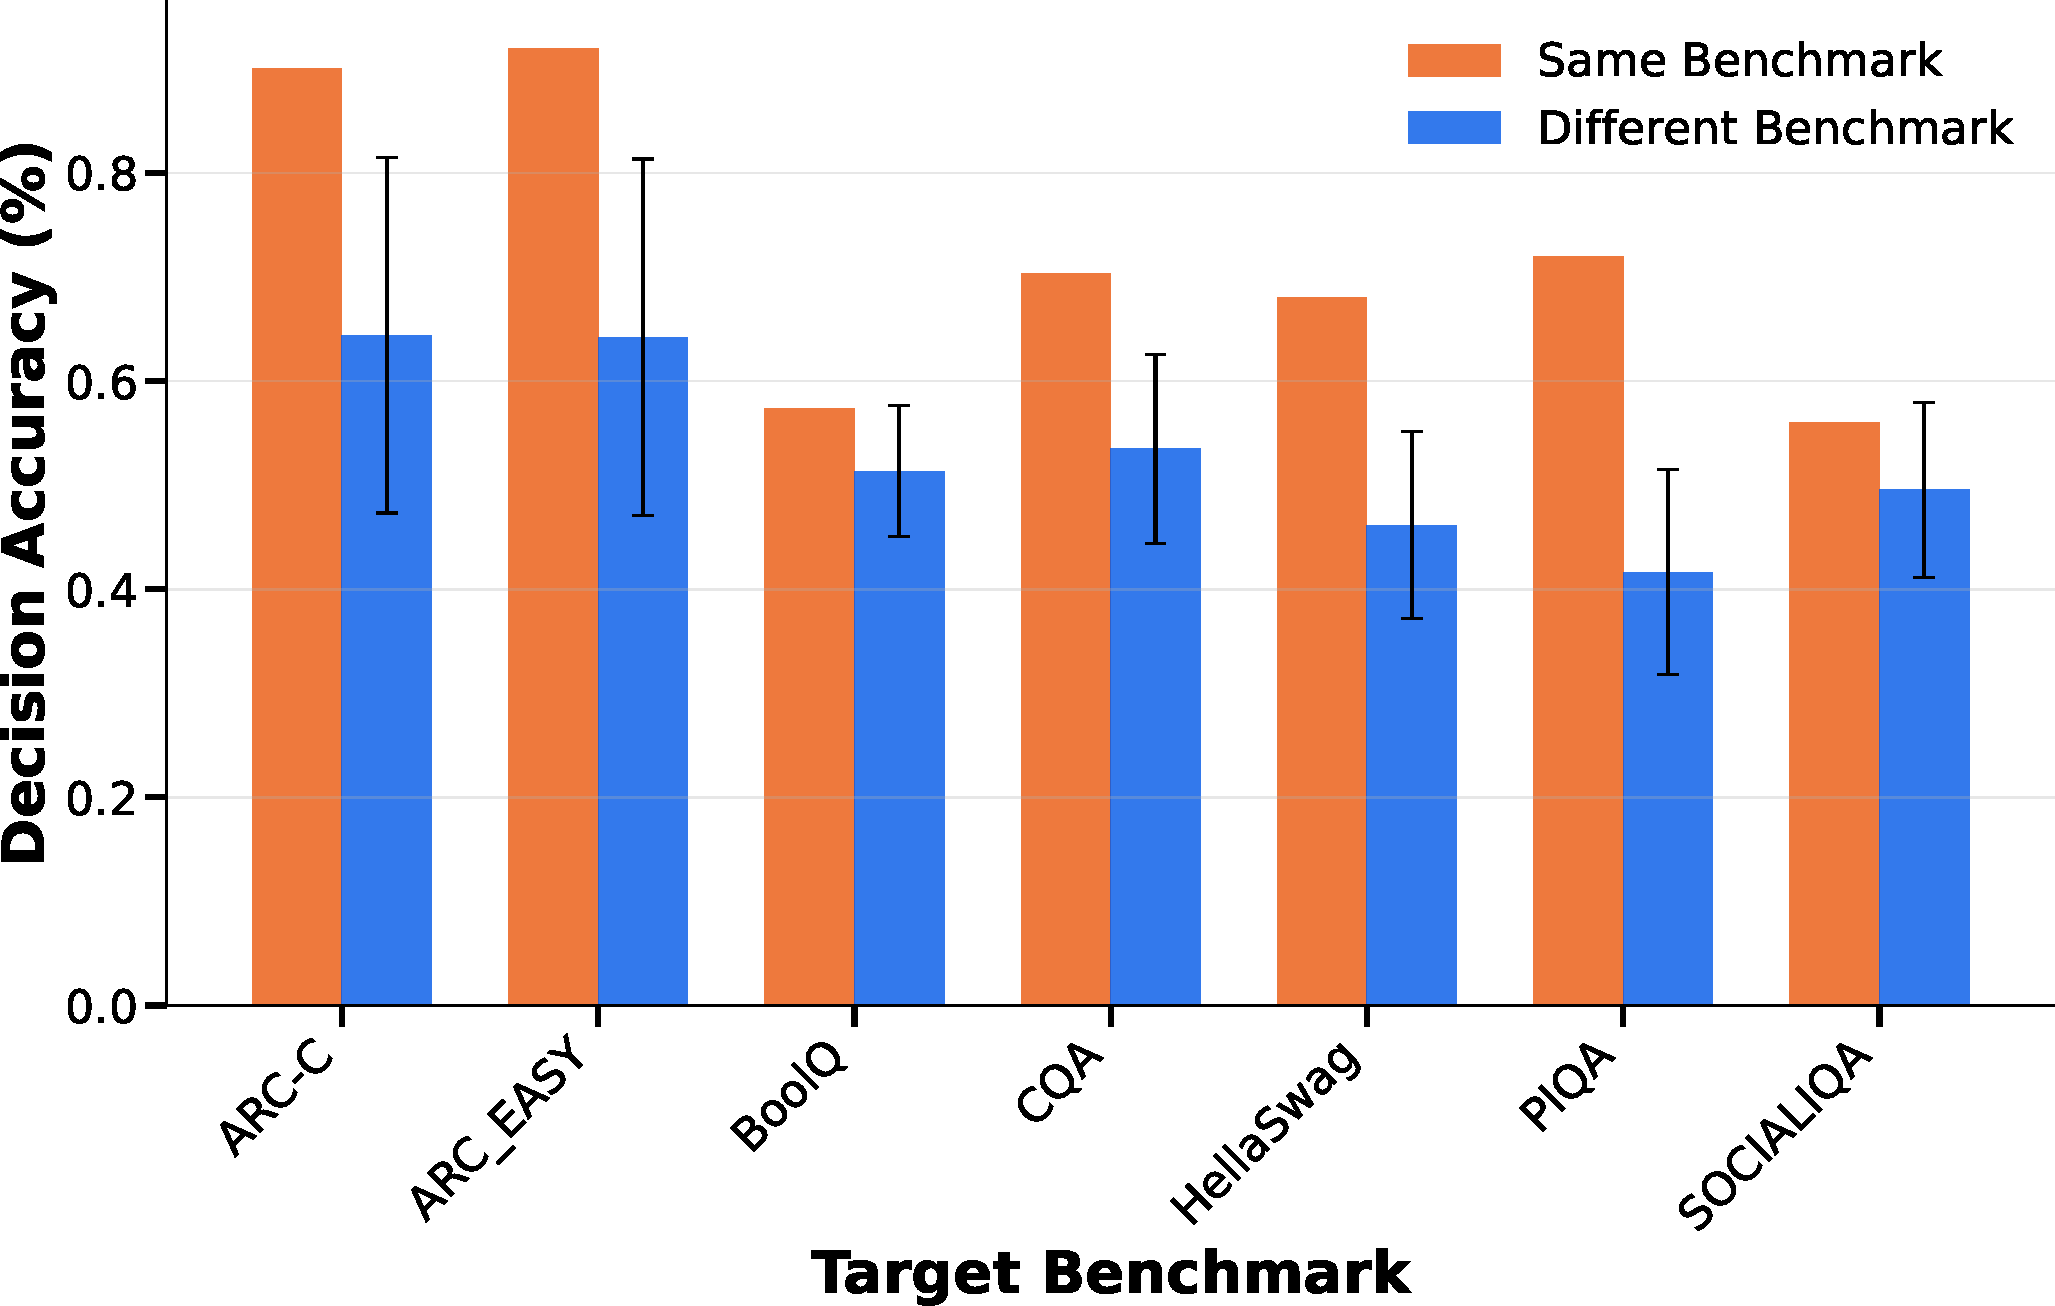
\includegraphics[width=\textwidth]{figs/benchmark_accuracy.pdf}
        \label{fig:proxy_acc}
    \end{subfigure}
    \caption{Correlation and decision accuracy performance using the same benchmark vs. different benchmark on 97.9M $\rightarrow$ 1.2B. Error bars indicate one standard deviation. On average, different benchmarks performs sub-optimally and are noisy.}
    \label{fig:proxytask}
\end{figure}

\section{Attribution} 

We attribute the neural network icon in Fig. \ref{fig:rbridge} as taken from Freepik (flaticon.com). Their guideline indicates that it can be used with attribution.
